\documentclass[12pt]{extarticle}

\usepackage{todonotes}
\usepackage{fontspec}
\usepackage{polyglossia}
\usepackage[a4paper, % Согласно требованиям к ВКР
  lmargin=30mm, rmargin=15mm, tmargin=20mm, bmargin=20mm]{geometry}
\usepackage{multirow}
\usepackage{amsmath,amssymb}
 % Required for including images

\DeclareRobustCommand{\bbone}{\text{\usefont{U}{bbold}{m}{n}1}}

\DeclareMathOperator{\EX}{\mathbb{E}}

\setdefaultlanguage{russian}
\setotherlanguage{english}


% Согласно требованиям к ВКР
\defaultfontfeatures{Ligatures=TeX}

\setmainfont{Times New Roman}
\setmonofont{Courier New}
\setsansfont{Arial}

\newfontfamily\cyrillicfont{Times New Roman}
\newfontfamily\cyrillicfontsf{Arial}
\newfontfamily\cyrillicfonttt{Courier New}

\newfontfamily\englishfont{Times New Roman}
\newfontfamily\englishfontsf{Arial}
\newfontfamily\englishfonttt{Courier New}

\linespread{1.5}

%\usepackage[dvipsnames]{xcolor}

%\renewcommand{\UrlFont}{\small\rmfamily\tt}


\renewcommand\thesection{\arabic{section}}

\usepackage{amsfonts}

\usepackage{tikz}
\usepackage{pgfplots}
\usepackage{wrapfig}


\usepackage{graphicx}
\graphicspath{ {./images/} }




\renewcommand*{\maketitle}{
\begin{titlepage}
  \begin{center}
    \linespread{1}
    \small
    Федеральное государственное автономное образовательное учреждение\break высшего образования\par
    <<Московский физико-технический институт \break (национальный исследовательский университет)>>\par
    Физтех-школа Прикладной Математики и Информатики\par
    Кафедра корпоративных информационных систем\par
  \end{center}
%
  {
    \small
    {\bf Направление подготовки / специальность}: 01.03.02 Прикладная математика и информатика\newline
    {\bf Направленность (профиль) подготовки}: Прикладная математика и компьютерные науки
  }
%
  {
    \topskip0pt
    \vspace*{\fill}
    \begin{center}
      {\bf\Large ИССЛЕДОВАНИЕ ИНФОРМАЦИОННОГО БЫТЫЛОЧНОГО ГОРЛЫШКА В НЕЙРОННЫХ СЕТЯХ}\par
      (бакалаврская работа)
    \end{center}
    \vspace*{\fill}
  }
%
  \hfill
  \begin{minipage}[t]{8cm}
    {\bf Студент: \newline}
    Николаев Михаил Алексеевич\newline
    \vspace{-3mm}
    \rule{8cm}{0.15mm}
    \centerline{\scriptsize\it (подпись студента)}\newline
%
    {\bf Научный руководитель: \newline}
    Леонидов Андрей Владимирович\newline
    \vspace{-3mm}
    \rule{8cm}{0.15mm}
    \centerline{\scriptsize\it (подпись научного руководителя)}
  \end{minipage}

    \vspace*{\fill}
    \begin{center}
      Москва 2022
    \end{center}
\end{titlepage}
}


\pgfplotsset{compat=1.18} 
\begin{document}
\maketitle

\newpage
\setcounter{page}{2}

\vspace*{\fill}
\begin{abstract}

Данная работа посвящена изучению  теории информации в нейронных сетях и исследованию Bottleneck Principe (принцип узкого места). В ходе работы была изучена взаимосвязь информации с алгоритмами машинного обучения на примере обучения нейронной сети классификации цифр по картинке.
\end{abstract}
\vspace*{\fill}
\newpage
\tableofcontents
\newpage
\section{Проблема}

\subsection{Введение}
Представим, что нам требуется обучить нейронную сеть. Будем рассматривать обучение с учителем. Тогда у нас есть вход $X$ и выход $Y$, во время обучения нейронной сети алгоритм пытается найти оптимальные веса, чтобы по входу $x_i \in X$ сеть получала выход $y_i \in Y$.  Нейронная сеть представляет собой последовательность слоев $\{Z_0, Z_1, Z_2, ..., Z_n\}$ где $Z_0 = X, Z_n = Y^'$,где $Y^'$ предсказание сети, и набор функций преобразований $\{f_1, f_2, ..., f_n\}$ и веса $\{\theta_1, \theta_2, ..., \theta_n\}$ , где $Z_{i+1}= f_i(Z_i, \theta_i)$. Соответственно сеть преобразовывает исходное пространство $X$ в латентное представление $Z$, которое является сжатым представлением пространства $X$. Это значит что у хорошей модели латентное пространство включает в себя всю необходимую информацию о входе для представления предсказания о выходе. То есть нам необходимо перенести из входа минимальное количество информации для латентного пространства для максимально подробного описания выхода. Эта оптимизационная задача называется принципом бутылочного горлышка. Хочется решить эту оптимизационную задачу и изучить как перетекает информация между слоями взависимости от качества сети.

\subsection{Формальная постановка задачи}
\begin{enumerate}
    \item Изучить литературу про теорию информацию в нейронных сетях, взять за основу данные о поведении информарционных метрик в течение обучении сети и использовать их как гипотезу.
    \item Взятие за основу легкую нейроннуй сеть (сеть классификации цифр по фото), построить алгоритм ее обучения.
    \item Подробно изучить логическое устройство каждого из пространсв, на основе этих знаний построить статистическую оценку для кажого слоя.
    \item Построение на ней множества вероятностных пространств - для каждого слой свое множество пространств. Каждое вероятное пространство задается гиперпараметрами.
    \item Построить распределение для каждого слоя, и совместные распределения между слоями.
    \item Посчитать информацинные метрики (такие как энтропия) на полученных распределениях.
    \item Посмотреть на полученные информационные метрики в зависимости от эпохи обучения, сравнить с гипотезами, полученными с помощью литературы
    \item Провести валидацию, на этапе которой подобрать наилучшие гиперпараметры вероятностных пространств и соответственно понять преимущества и недостатки каждого из вероятностных пространств.
    \item Сделать выводы о проведенных экспериментов.
\end{enumerate}
\newpage

\section{Обзор литературы}
\subsection{Базовые определения}
Рассотротрим вероятностное просранство $(X, \Theta, p)$, где $X$ просранство, $\Theta$ сигма- алгебра на $X$, $p$ вероятносная мера введеная на сигма-алгебре $\Theta$.
Тогда введем энтропию
\begin{gather}
\begin{aligned}  
H[X] = - \EX_{p(x)}\log(p(x))
\end{aligned}
\end{gather}
В дискретном случае
\begin{gather}
\begin{aligned}  
H[X] = - \sum_{x \in X}p(x)\log(p(x))
\end{aligned}
\end{gather}
Введем совместную энтропию
\begin{gather}
\begin{aligned}  
H[X, Y] = - \EX_{p(x, y)}\log(p(x, y))
\end{aligned}
\end{gather}
В дискретном случае
\begin{gather}
\begin{aligned}  
H[X, Y] = - \sum_{x \in X, y \in Y}p(x, y)\log(p(x, y))
\end{aligned}
\end{gather}
Теперь введем условную энтропию
\begin{gather}
\begin{aligned}  
    H[X | Y] = - \EX_{p(x, y)}\log(p(x | y)) = H[X, Y] - X[Y] \\
\end{aligned}
\end{gather}
\begin{gather}
\begin{aligned}
    \Box \: H[X, Y] - X[Y] = - \EX_{p(x, y)}\log(p(x, y)) + \EX_{p(y)}\log(p(y)) =  \\
    - \int_{x, y}p(x, y)\log(p(x, y)) + \int_{y}p(y)\log(p(y)) = \\
    - \int_{x, y}p(x, y)\log(p(x, y)) + \int_{y}\sum_{x}p(y, x)\log(p(y)) = \\ 
    - \int_{x, y}p(x, y)\log(p(x, y)) + \int_{x, y}p(y, x)\log(p(y)) = \\ 
    - \int_{x, y}p(x, y)(\log(p(x, y)) - \log(p(y))) = \\ 
    - \int_{x, y}p(x, y)(\log(p(x, y) / p(y))) = - \int_{x, y}p(x, y)\log(p(x | y)) = H[X | Y] \:\Box
\end{aligned}
\end{gather}    
Теперь введем информацию между двумя величинами
\begin{gather}
\begin{aligned}
    I[X, Y] = - \EX_{p(x, y)}\log(\frac{p(x)p(y)}{p(x, y)}) = H[X] + H[Y] - H[X, Y]
\end{aligned}
\end{gather}    
\begin{gather}
\begin{aligned}
    \Box \: H[X] + H[Y] - H[X, Y] = \\ 
    - (\int_{x, y}p(y, x)\log(p(x)) + \int_{x, y}p(x, y)\log(p(y)) - \int_{x, y}p(y, x)\log(p(x, y))) = \\
    - \int_{x, y}p(y, x) (\log(p(x)) + \log(p(y)) - log(p(x, y))) = \\
    - \int_{x, y}p(x, y)\log(\frac{p(x)p(y)}{p(x, y)}) = I[X, Y] \:\Box 
\end{aligned}
\end{gather}    
\subsection{Информационные множества}
Таким образом информационные эвристики можно воспринимать как множественные операции
\begin{center}
    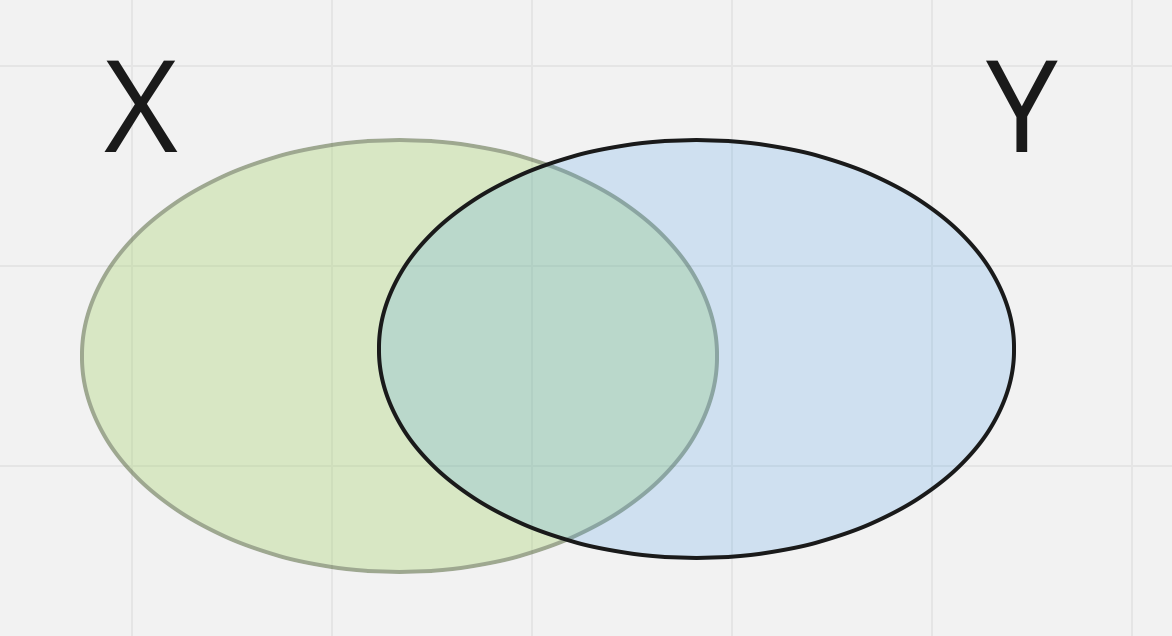
\includegraphics[scale=0.4]{images/information_sets.png}
\end{center}
Рассмотрим пространства $X$ и $Y$ как множества, тогда мощностью множества
\begin{enumerate}
\item $|X|$ будем называть $H[X]$
\item $|Y|$ будем называть $H[Y]$
\item $|X \cap Y|$ будет $I[X, Y]$
\item $|X \cup Y|$ будет $H[X, Y]$
\item $|X \setminus Y|$ будет $H[X | Y]$
\item $|Y \setminus X|$ будет $H[Y | X]$
\end{enumerate}
Перейдем к рассмотрению информационных множеств в рамках нейронных сетей. Тогда $X$ рассмотрим как пространство входных данных, $Y$ рассмотрим как пространство выходных данных, $Z$ как латентное пространство. Визуализируем их в качестве множеств. Подобная диаграмма называется Mickey Mouse I-diagram.
\begin{center}
    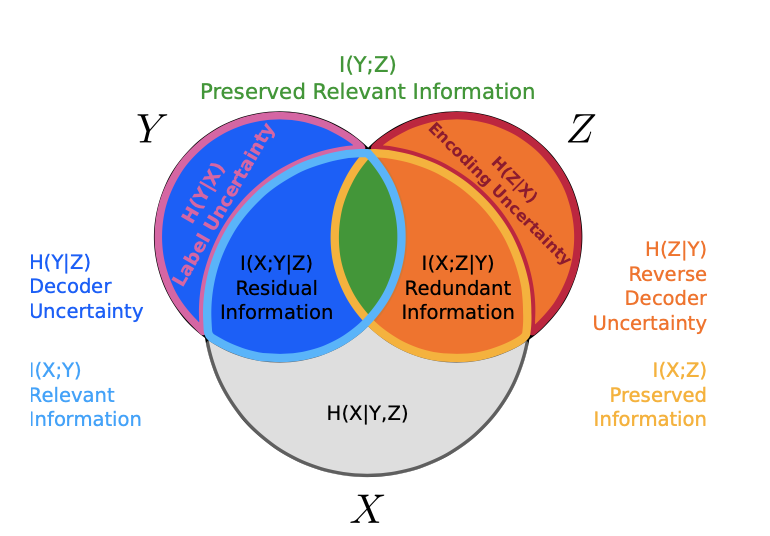
\includegraphics[scale=1.]{images/micky_mouse_diagram.png}
\end{center}
Соответственно каждое из подмножеств численно вычисляется с помощью информационных метрик. Заметим, что $X \cap Y \cap Z = Y \cap Z$, иными словами $I[X, Y, Z] = I[Y, Z]$. Докажем это. $I[X, Y, Z] = I[Y, Z] \Leftrightarrow I[Y, Z] - I[X, Y, Z] = H[Y, Z | X] = 0$. Это верно, так как для каждого входа $x_i \in X$ зафиксирован конкретный выход $y_i \in Y$ и конкретное латентное кодирование $z_i \in Z$, а значит пространство $(Y, Z | X)$ будет одномерно для каждого $x_i \in X$, следовательно $H[Y, Z | X] = 0$.
\subsection{Information Bottleneck Principe}
Задача нейронной сети вычленить всю релевантую информацию из входа $X$ описывающую выход $Y$. Оптимальное отображение будет отбрасывать всю нерелевантную информацию, таким образом задача обучения состоит в том, чтобы минимизировать общую информацию $I[X, Z]$, при этом сохраняя всю необходимую общую информацию между выходом и латентным пространством $I[Y, Z]$. Обощая эти факты, поиск оптимального решения описывается задачей оптимизации (IB):
\begin{gather}
\begin{aligned}
min_{Z} I[X, Z] - \beta * I[Z, Y]
\end{aligned}
\end{gather}
Где $\beta$ оператор компромиса между информацией репрезентации $I[X, Z]$, и информацией релевантной информации $I[Z, Y]$. Посмотрев на Mickey Mouse I-diagram можно заметить, что множество $Z$ пытается максимально влится в $Y$ и иметь наименьшее пересечение с $X$. Проверим данные гипотезы на практике.









\newpage
\section{Архитектура нейронной сети}
\subsection{Описание задачи и датасета}
В качестве примера возьмем нейронную сеть класификации цифр по картинке. За основу датасета возьмем MNIST датасет. В датасете педставлены чернобелые картинке рукописных цифр и соответсвующие им значения цифр, которые представлены на картинке. На каждом изображении изображена ровно одна цифра. Датасет разделен на 2 части: train и test для тестирования и обучения. Для практики выбрана такая задача, так как сеть для обучения получится легкой: в ней будет мало параметров, сеть обучается довольно быстро и за небольшое количество эпох, также данная задача хорошо подходит для исследования, так как на вход подается картинка, это пространство имеет размерность матрицы, на выходе же подается число, размерность которого одномерная. Соответственно в ходе преобразований сеть должна выявить все релевантные признаки и сильно сжать пространство, что полезно для нашего эксперимента.

\subsection{Архитектура сети}
Количество семплов в обучающей выборке 6000, размер каждого изображения (28, 28). Изображение одноканальное, так как оно чернобелое. Сеть предствляет собой следующую архитектуру
\begin{center}
    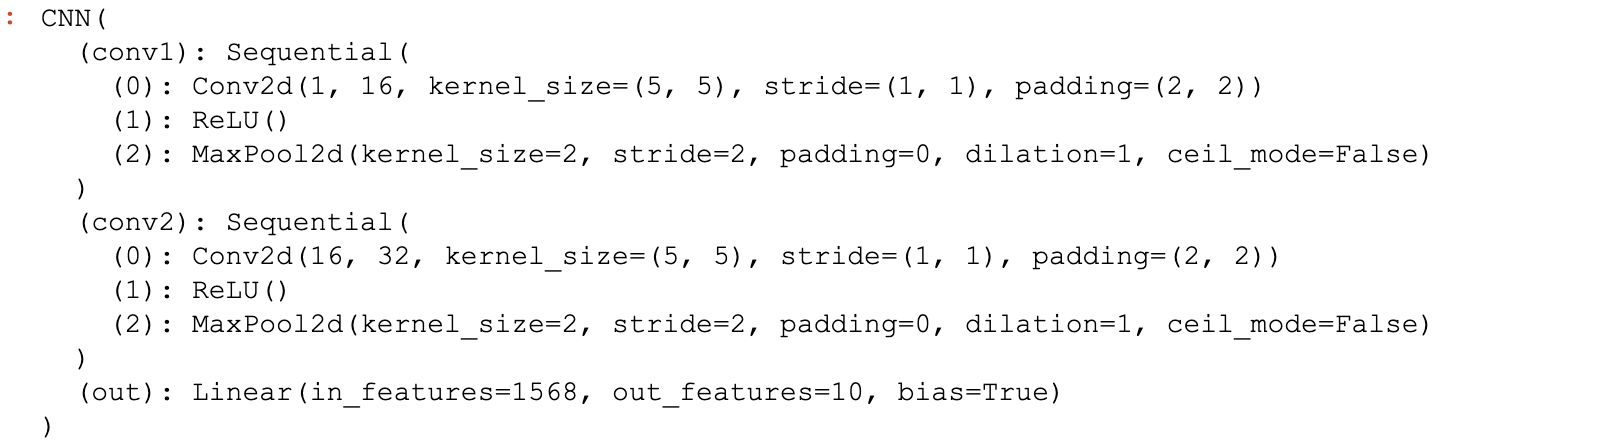
\includegraphics[scale=0.7]{images/CNN_arciticture.png}
\end{center}
Подробная количественная таблица параметров сети:
\begin{center}
    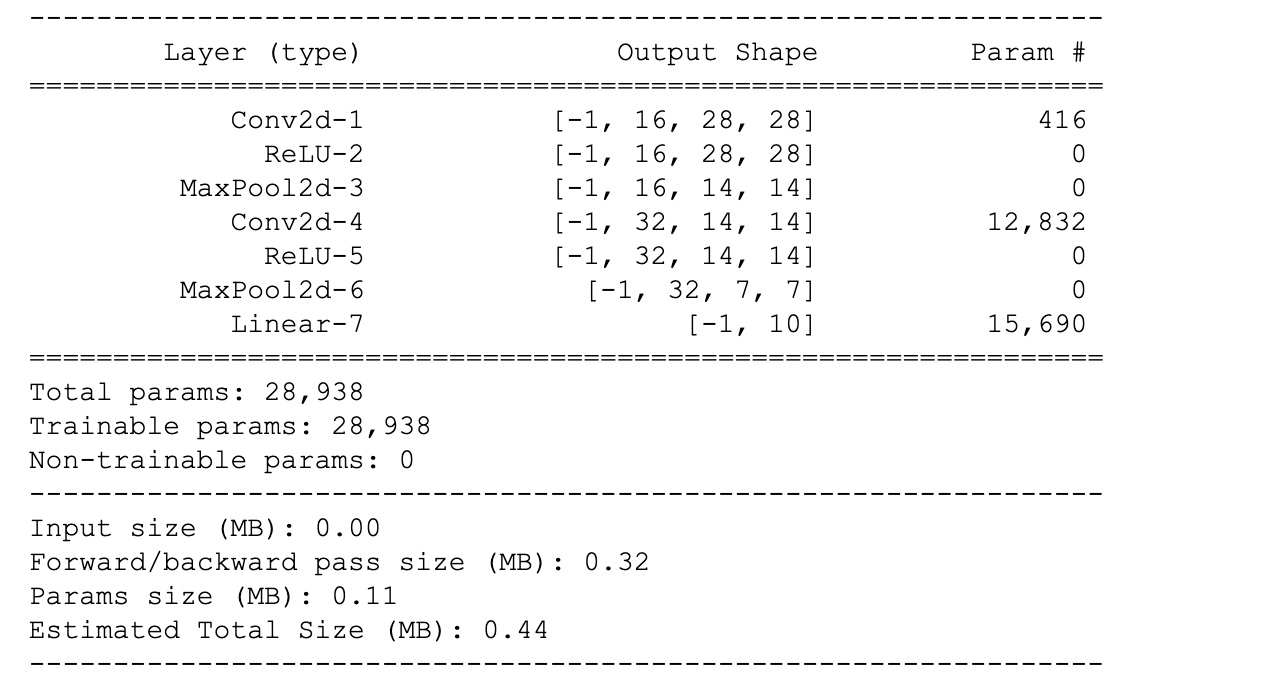
\includegraphics[scale=0.7]{images/cnn_params.png}
\end{center}
Соответственно сеть начинается с  2 сверточных слоев (conv1, conv2). Свертки представляют собой последовательность: 2d-свертка, функция архивации (ReLU()) и пуллинг (MaxPool2d). Далее после последововательных применений сверток conv1 и conv2 к входному тензору, тензор транспонируется в двумерный тензор, далее к нему применяется полнозвязный слой и функция Softmax. Финальное представление должно предсказывать вероятностное распределение на цифрах. \\
\subsection{Цикл обучения сети с подробным forward pass}
\begin{enumerate}
    \item $z_1 = conv1(x)$, где $x$ - входной батч, conv1 - первая свертка. $x.shape = (batch\_size, 1, 28, 28)$
    \item $z_2 = conv2(z_1)$, где $z_1$ - выход первого слоя сети, иначе говоря первого латентного пространства, conv2 - вторая свертка. $z_1.shape = (batch\_size, 16, 28 / 2, 28 / 2)  = (batch\_size, 16, 14, 14)$.
    \item $z_2^{flatten} = flatten(z_2)$, где $z_2$ - выход второго слоя сети, $flatten$ - функция меняющая размерность тензора, а именно превращая все признаки в одномерное векторное пространство. $z_2.shape = (batch\_size, 32, 14 / 2, 14 / 2) = (batch\_size, 32, 7, 7)$.
    \item $z_3 = linear(z_2^{flatten})$, где $z_2^{flatten}$ - выход второго одномерного слоя сети, $linear$ - полносвязный слой. $z_2^{flatten}.shape = (batch\_size, 32 * 7 * 7) = (batch\_size, 1568)$.
    \item $target = softmax(z_3)$, где $z_3$ - выход третьего слоя, функция softmax позволяет репрезентовать распределение, как вероятностное распределение в отрезке $[0, 1]$, $z_3.shape = (batch\_size, 10)$ 
    \begin{gather}
    \begin{aligned}
    softmax(x_i) = \exp(x_i) \setminus (\sum_{j}\exp(x_j))
    \end{aligned}
    \end{gather}
    \item Выход $y$ представляется как one hot вектор $y_{onehot}$, например 
    \begin{gather}
    \begin{aligned}
    y = 3 \Leftrightarrow y_{onehot} = [0, 0, 0, 1, 0, 0, 0, 0, 0, 0]
    \end{aligned}
    \end{gather}
    \item $y_{onehot}$ сравнивается с $target$ с помощью лосс функции кросс энтропии $L$
    \begin{gather}
    \begin{aligned}
    L(y, t) = - \sum_{i}y_i * \log(t_i)
    \end{aligned}
    \end{gather}
\end{enumerate}
Данная сеть обучалась с помощью инфмационной метрики в лоссе - кросс энтропии между таргетом и ground truth. При этом не учитывались никакие другие информационные эвристики в других латентных пространствах ($z_1, z_2, z_3)$.




\newpage
\section{Вероятностное пространство}

Для работы с информационными эвристиками нам нужно построить вероятностное пространство для каждого слоя. Пространства входа $X$ и выхода $Y$ не изменяются в зависимости от эпохи обучения. При этом латентное пространство $Z$ будет менятся с каждыми новыми весами моделей. \\
\subsection{Вероятностное пространство на выходном слое}
Проше всего задать вероятностное пространство на выходном слое, так как это категоричный признак, он принимает только целые числа в отрезке [0, 9]. Cоотвенственно если данные в семплах распредены равномерно, то вероятность выпадания каждого класса - 0.1. проверим это посчитав количествено все метри на датасете.
\begin{center}
    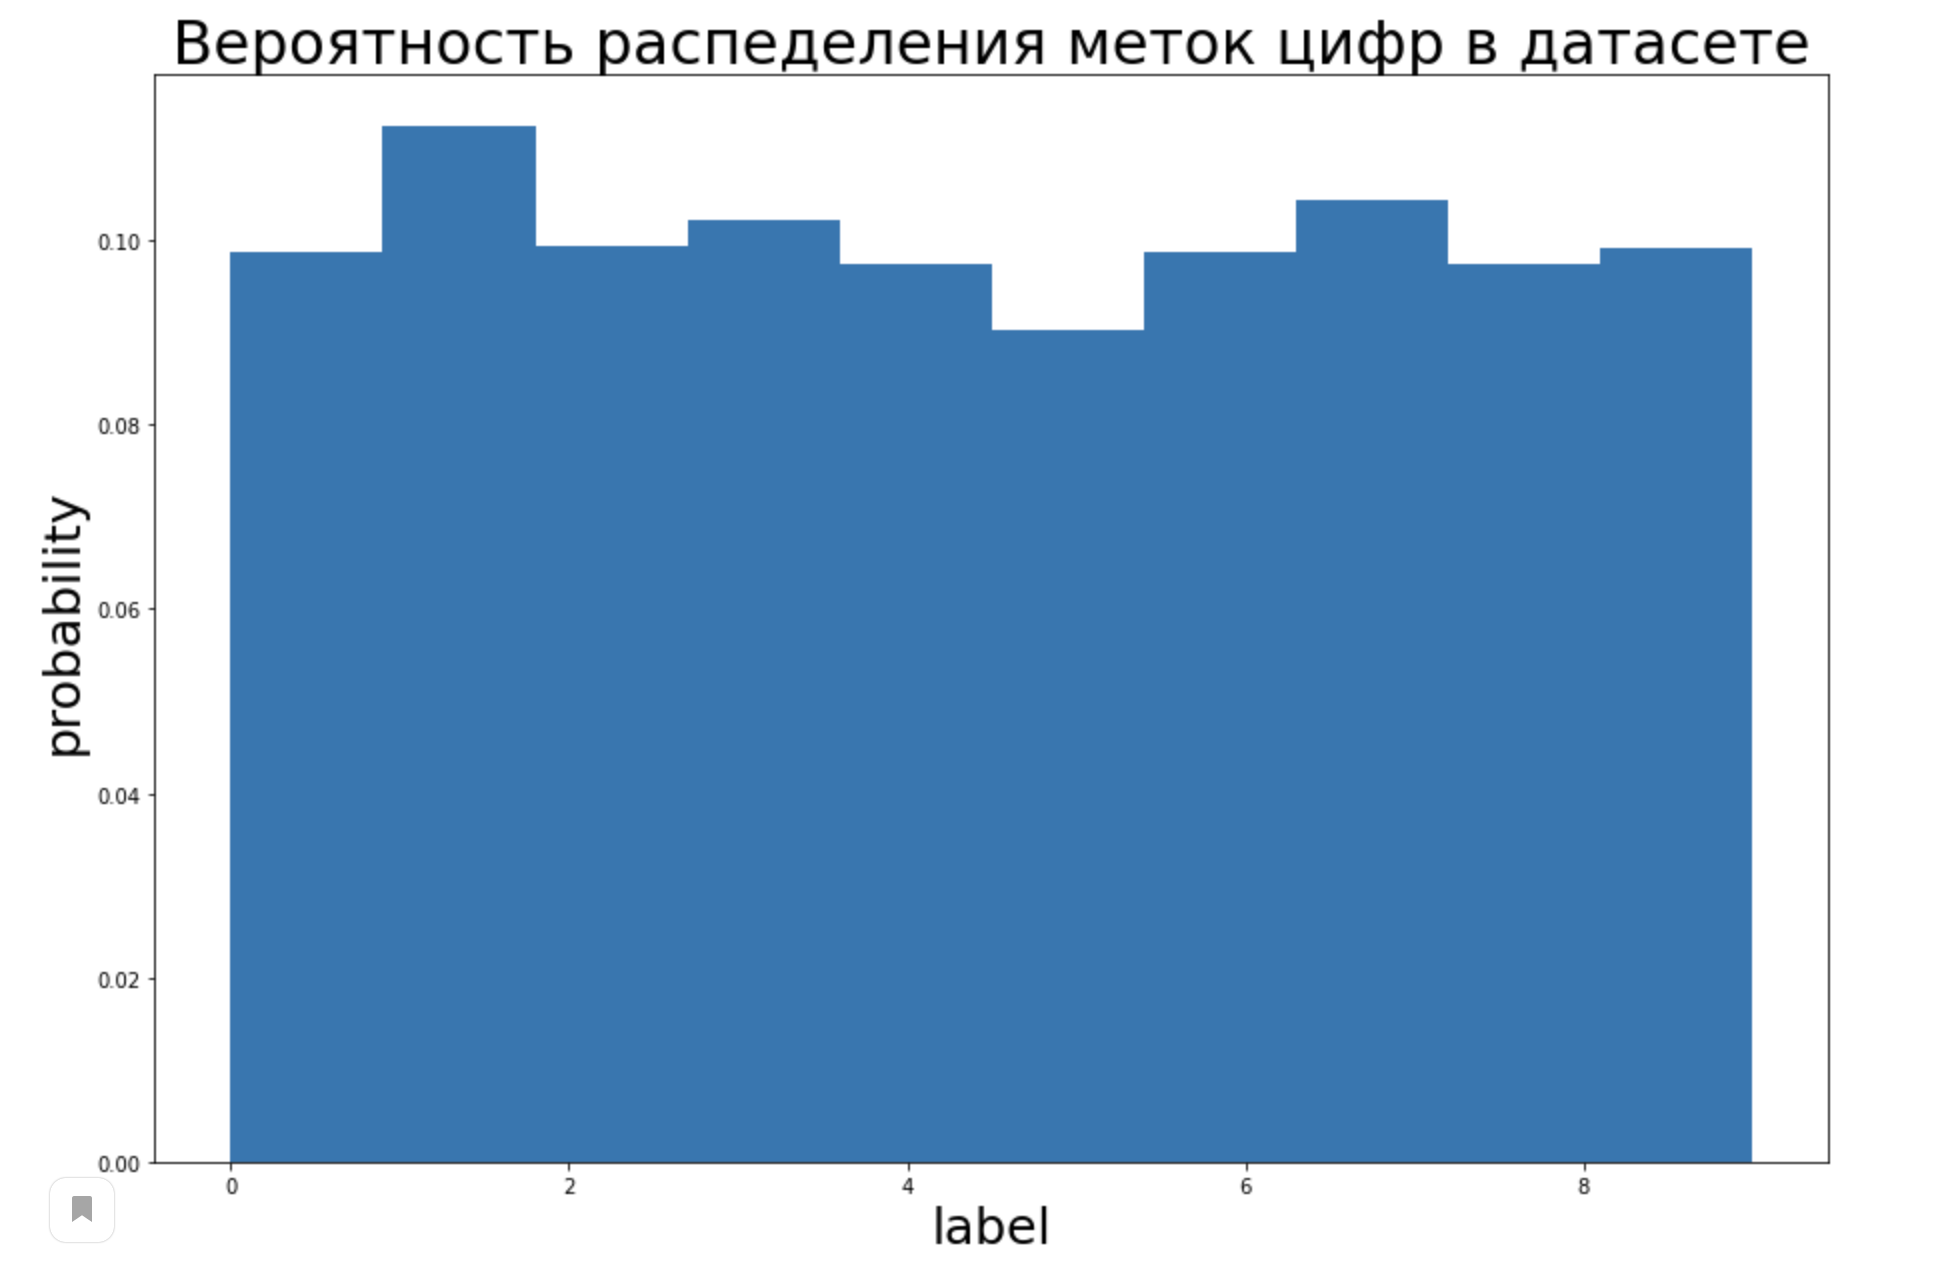
\includegraphics[scale=0.4]{images/y_prob.png}
\end{center}
Как видно на графике распределение на выходном слое почти равномерное, будем считать что вероятность для каждого элемента будет 1 / 10.
Сложнее ситуация с пространства входа и латентными, так как они многомерные.
\subsection{Вероятностное пространство на входном слое}
Сначала разберемся с входным пространством. Его размерность $(samples\_count, 1, 28, 28)$. Рассмотрим конкретную координату картинки и посмотрим как распределены значения на конкретном признаке. \\
В качестве примера возьмем координаты (14, 14) и (7, 7):
\begin{center}
    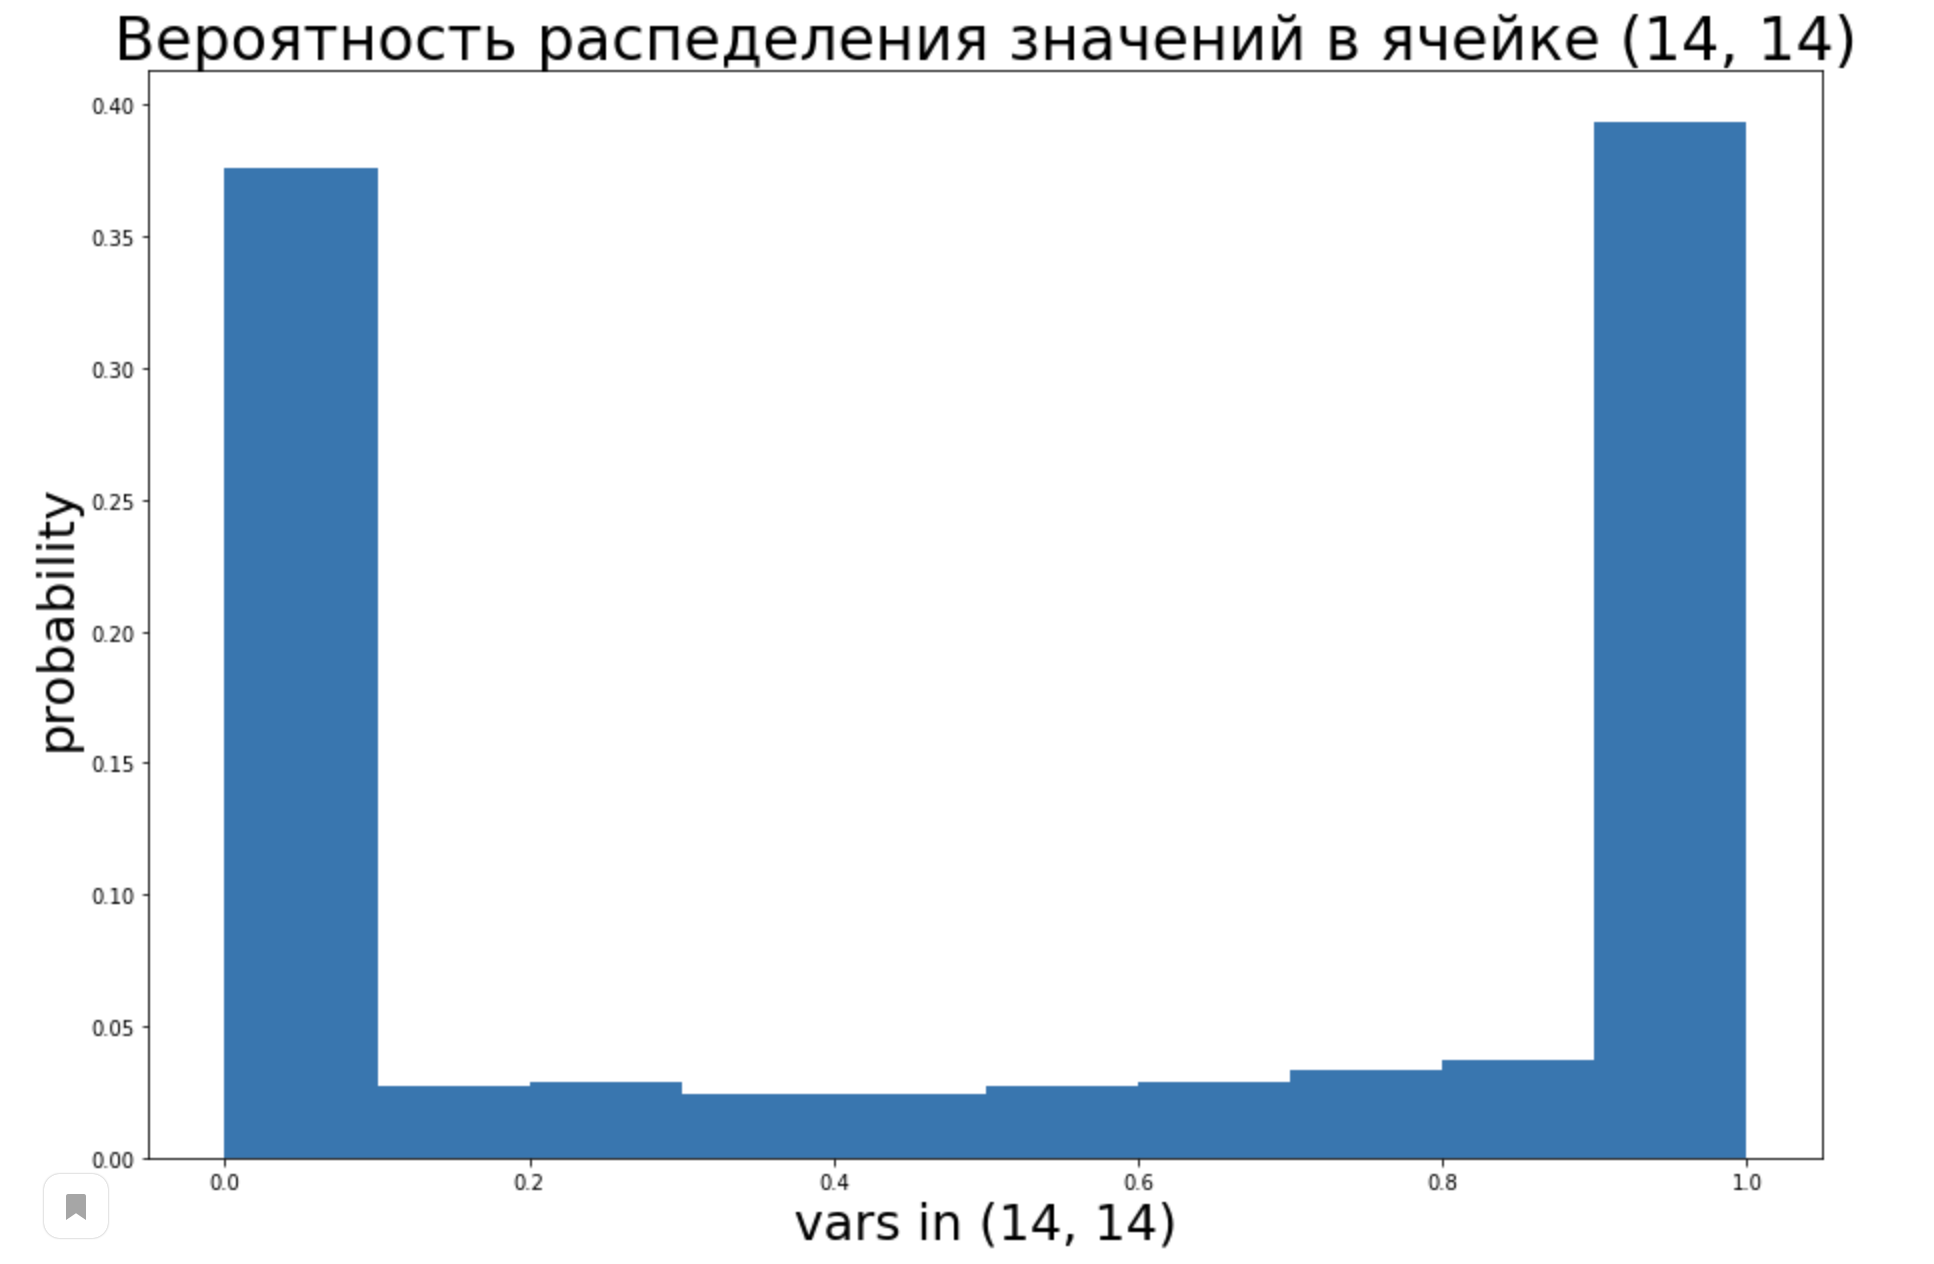
\includegraphics[scale=0.4]{images/x_(14, 14).png}
\end{center}
\begin{center}
    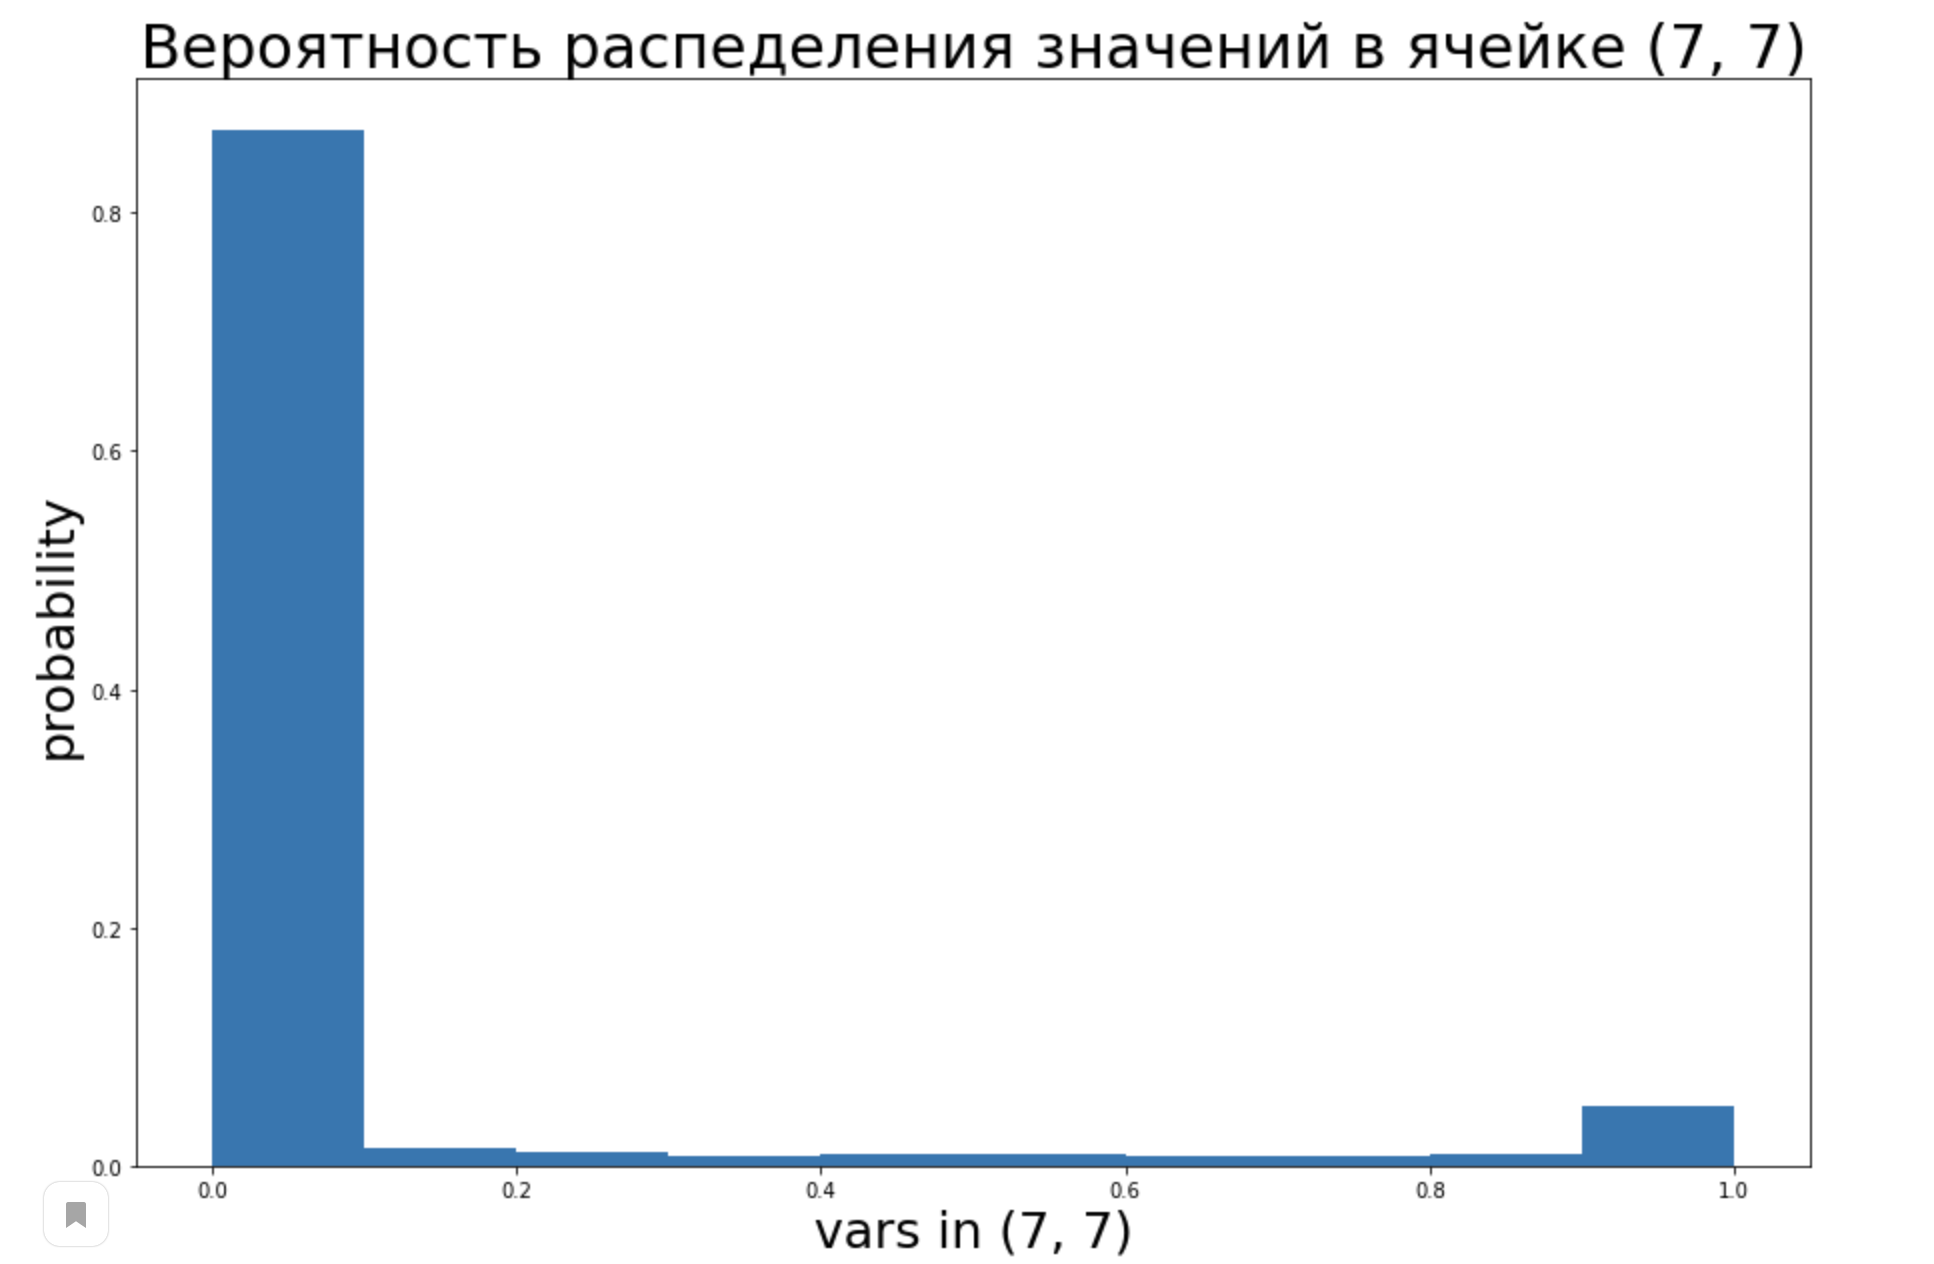
\includegraphics[scale=0.4]{images/x_(7, 7).png}
\end{center}
Видно, что значения внутри каждой ячейки распределены нестандартно, привалирующие значения - 0 и 1. Также правильнее рассматривать модель, где значения в каждой ячейке зависят друг от друга, так как картинки являются не случайным шумом, а непрерывными матрицами, то есть если все значения вокруг ячейки равно 1., то скорее всего значение в ячейки тоже 1. Проверим этот факт независимости. \\
Возьмем квадратик из 4 ячеек и проверим вероятность условия, что все значения больше 0.5 и также посчитаем перемноженную вероятность что значение в каждой ячейке больше 0.5 и сравним эти значения
\begin{gather}
\begin{aligned}  
P(x_{i,j} > 0,5, x_{i,j+1} > 0,5, x_{i+1,j} > 0,5, x_{i+,j+1} > 0,5) \\
? \\
P(x_{i,j} > 0,5), * P(x_{i,j+1} > 0,5) * P(x_{i+1,j} > 0,5) * P(x_{i+,j+1} > 0,5)
\end{aligned}
\end{gather}
Рассмотрим конкретный пример, описанный выше со значениями i = 14, j = 14
\begin{center}
    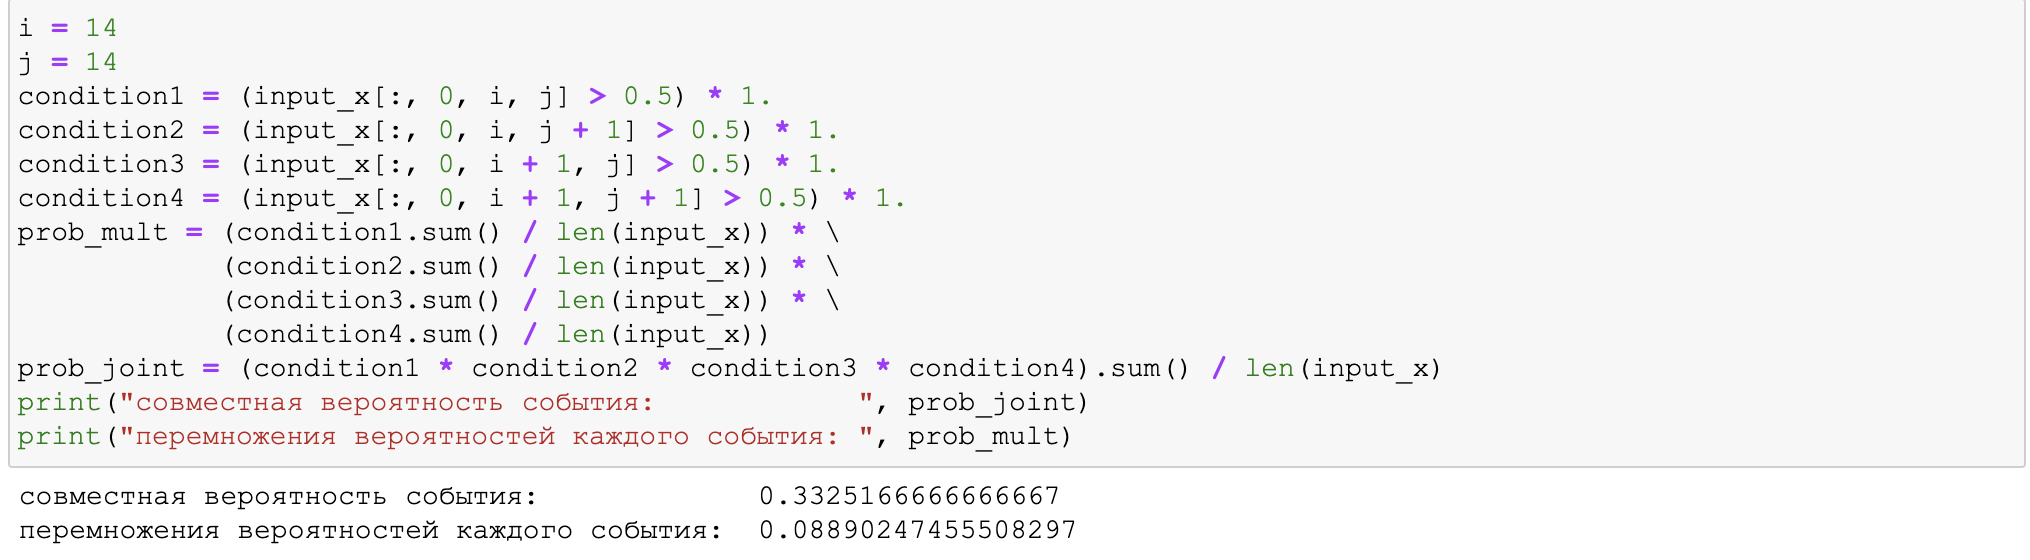
\includegraphics[scale=0.6]{images/x_independency.png}
\end{center}
Как видно на примере значения совершенно различные что говорит о зависимости между признаками входа. \\
Для удобства дискретизируем все значения входа, так как значения на входе принимают вещественные значения на отрезке [0, 1]. Четкое количество кусков разбиения оставим в качестве гиперпараметра и подберем при валидации. При дикретизации мы будем иметь дело с конечным пространством, что удобнее. Пример такой дискретизации:
\begin{gather}
\begin{aligned}  
X_{discrete} = (X_{input} > 0.5) * 1.
\end{aligned}
\end{gather}
Данная дискретизация приводит все значения к двум полярным - 0 и 1, данная дикретизация нам подходит, так как на примерах распределения значений по признакам значения с наибольшими вероятностями были именно полярные значения. \\
На данный момент непонятно какими вероятнострыми моделями приближать такие сложные многомерные пространства как входное, поэтому наилучшим решением будет рассматривать исходы как элементы построенного дискретного пространства. Может быть проблема, что каждый элемент датасета будет инъективно отображаться в построенное дискретное пространства, для проверки этого посчитаем количество различных исходов. Пусть количество параметров при дискретизации будет минимально, а именно 2. То есть все входные значения переходят либо в 0 либо в 1. В таком случае полученное пространство будет иметь $2^{28*28}$ различных исходов, тем временем количество элементов в датасете 60000, что на много порядков меньше чем $2^{28*28}$. Для решение этой проблемы используем искуственное сжатие пространства, которое рассмотрим чуть позже.
\subsection{Вероятностное пространство на латентных пространствах}
Для начала посмотрим как устроены данные на промежуточных слоях. Это также многомерные пространства, посмотрим на пример распределения одного из признаков слоя после первой свертки:
\begin{center}
    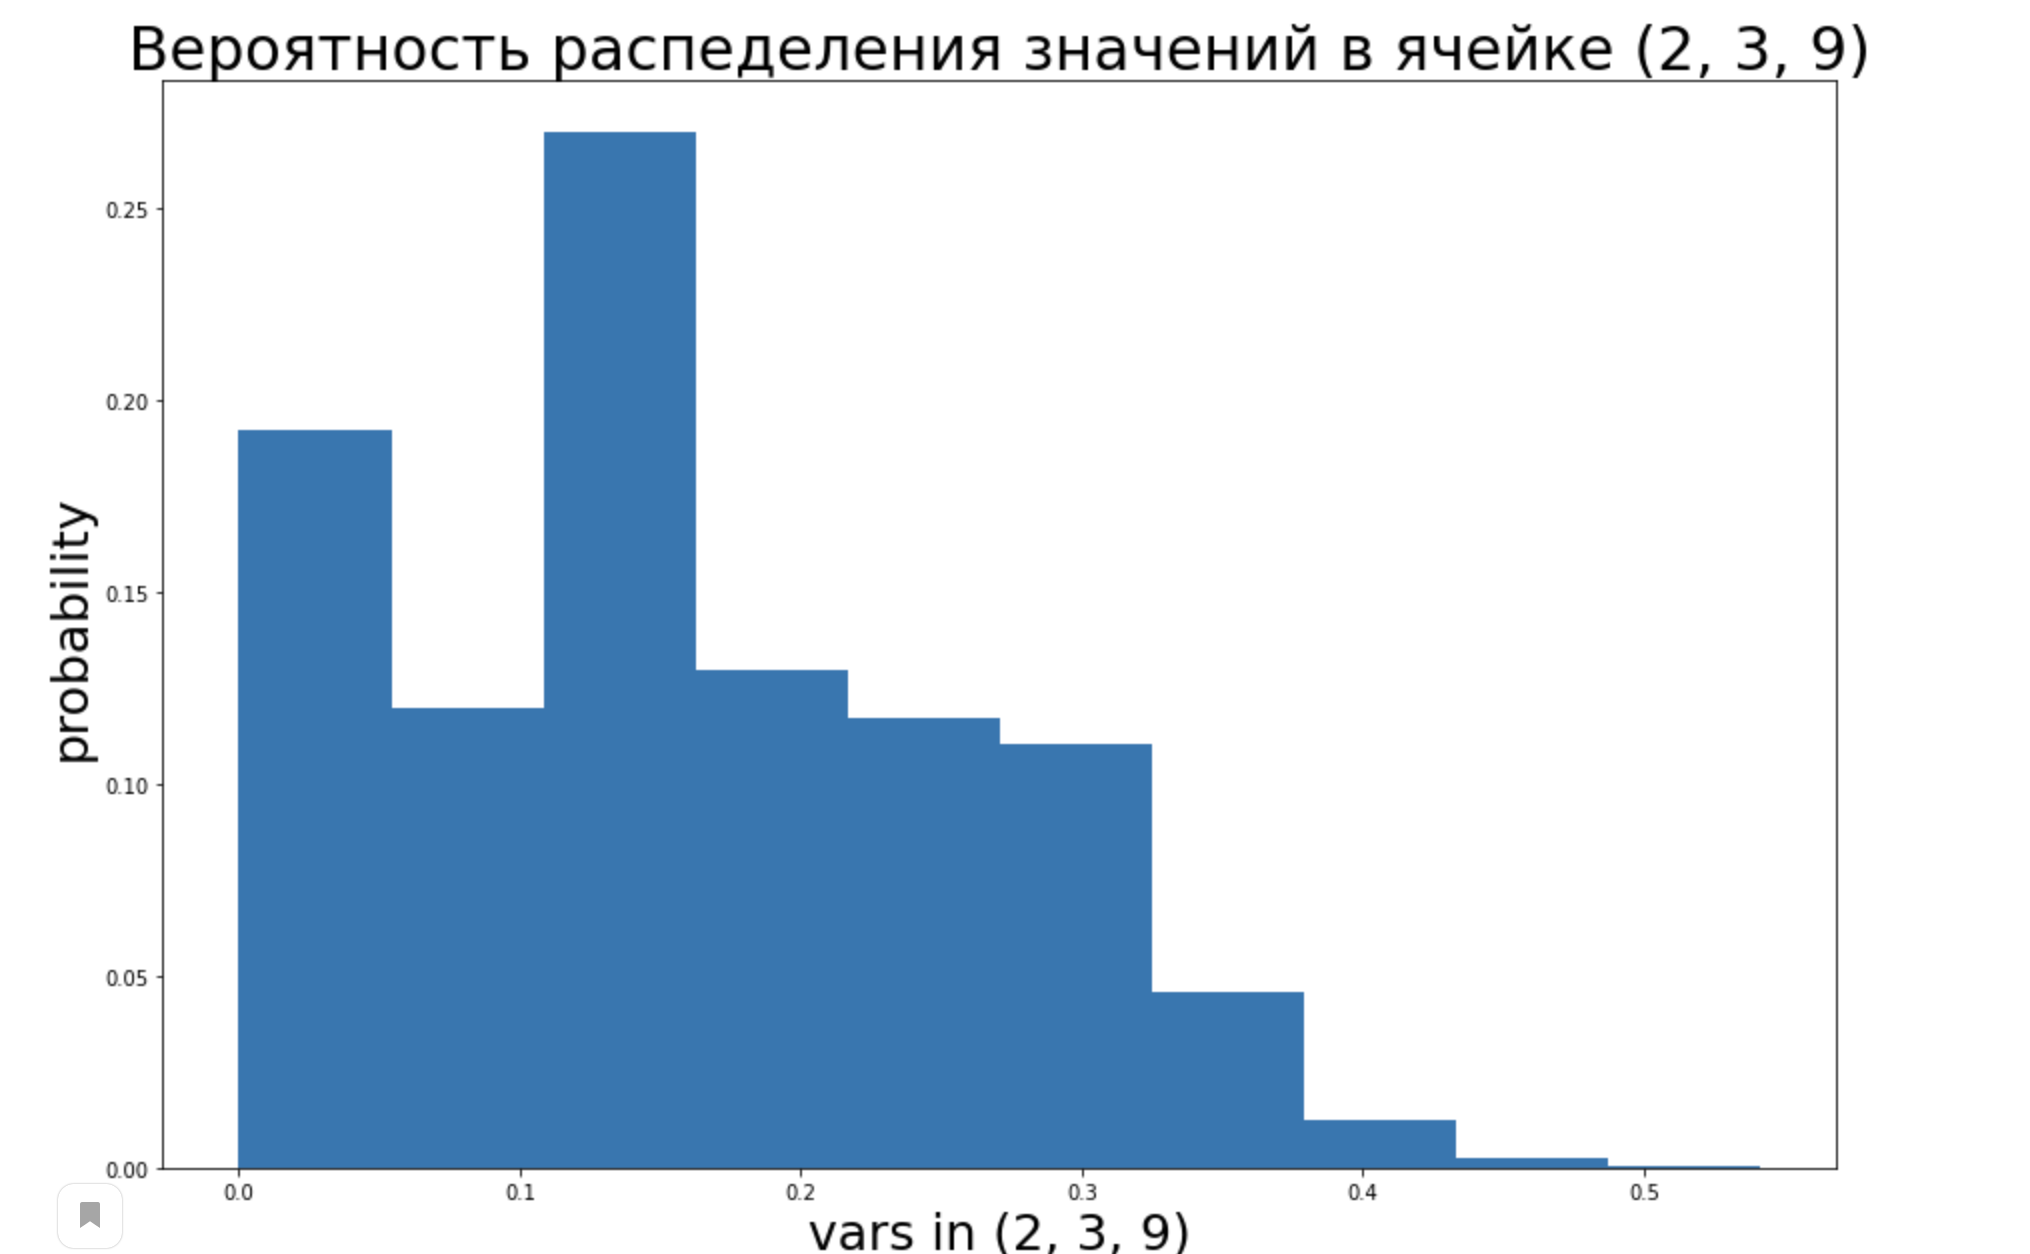
\includegraphics[scale=0.4]{images/Z1_dist.png}
\end{center}
Данные здесь получаются после применения 2d свертки, ативации RELU и после пуллинга, соответственно все данные меньшие 0 стали равны 0, можно сделать вывод что после сверки данные имели нормальное распределение с шумом, но после функции активации стали иметь распределение как у функции RELU(norm), описать стандартной моделью подобные данные не получится. \\
Также данные будут зависимы друг с другом по призакам, так как значения в латентных слоях являются функцией от входных данных, которые выполняются на forward pass. Так как forward pass будет работать почти инвариантно на первых слоях сети из-за больших размеров пространств зависимость созраняется. \\
Соответственно для построения латентного пространства мы также проводим дискретизацию, чтобы привести непрерывное пространство в конечное. Для этого мы находим квантили распределения (например 0.01 и 0.99 квантиль) и ограничиваем нашу область по признаку этой квантилью. Значения будут находится за ее пределами с вероятностью $0.01 + (1 - 0.99) = 0.02$. Далее разбиваем полученный отрезок на несколько равномерных кусков и дискретизируем. Количество кусков оставим в качестве гиперпараметра и подберем его при валидации. \\
При расчете полученного пространства после дискретизации возникают те же проблемы, что и на входном пространстве. Если рассматривать в качестве исходов - элементы дискретизации, то распределение получится также равномерным в силу того, что количество семплов в датасете намного меньше чем возможных вариантов исходов, поэтому прибегнем к такому же сужению пространства, поговорим про него поподробней.
\subsection{Сужение вероятностных пространств}
Как выяснилось в предъидущих пунктах, работать с вероятностным пространством без сужения будет бессмысленно, покажем это на практике в главе ниже. \\
Для снижения пространства будем использовать пуллинги, то есть объединение соседних признаков тензора в один. Эта операция сохраняет вероятно-признаковое пространство, так как в архитектурах сети часто используются пуллинги (как например в нашей сети классификации цифр по картинке). Особенности пуллинга также будем использовать как гиперпараметр. \\
Для двумерного пространсва такого как нащи исходные данные будем использовать $2d average pooling$. Если использовать окно 7x7 то после 
пуллинга размер матрицы будет $(28 / 7) * (28 / 7) = 16$. В таком случае количество исходов полученного вероятностного пространства будет $2^{16} = 65538$, что уже сопоставляется с размерностью исходного датасета. Уже в этом случае 
\begin{gather}
\begin{aligned}  
p(f(x_i) = f(x_j) \cap i \neq j) \ll 1, \\
f = discrete \circ pooling 
\end{aligned}
\end{gather}
Пример 2d пуллинга:
\begin{center}
    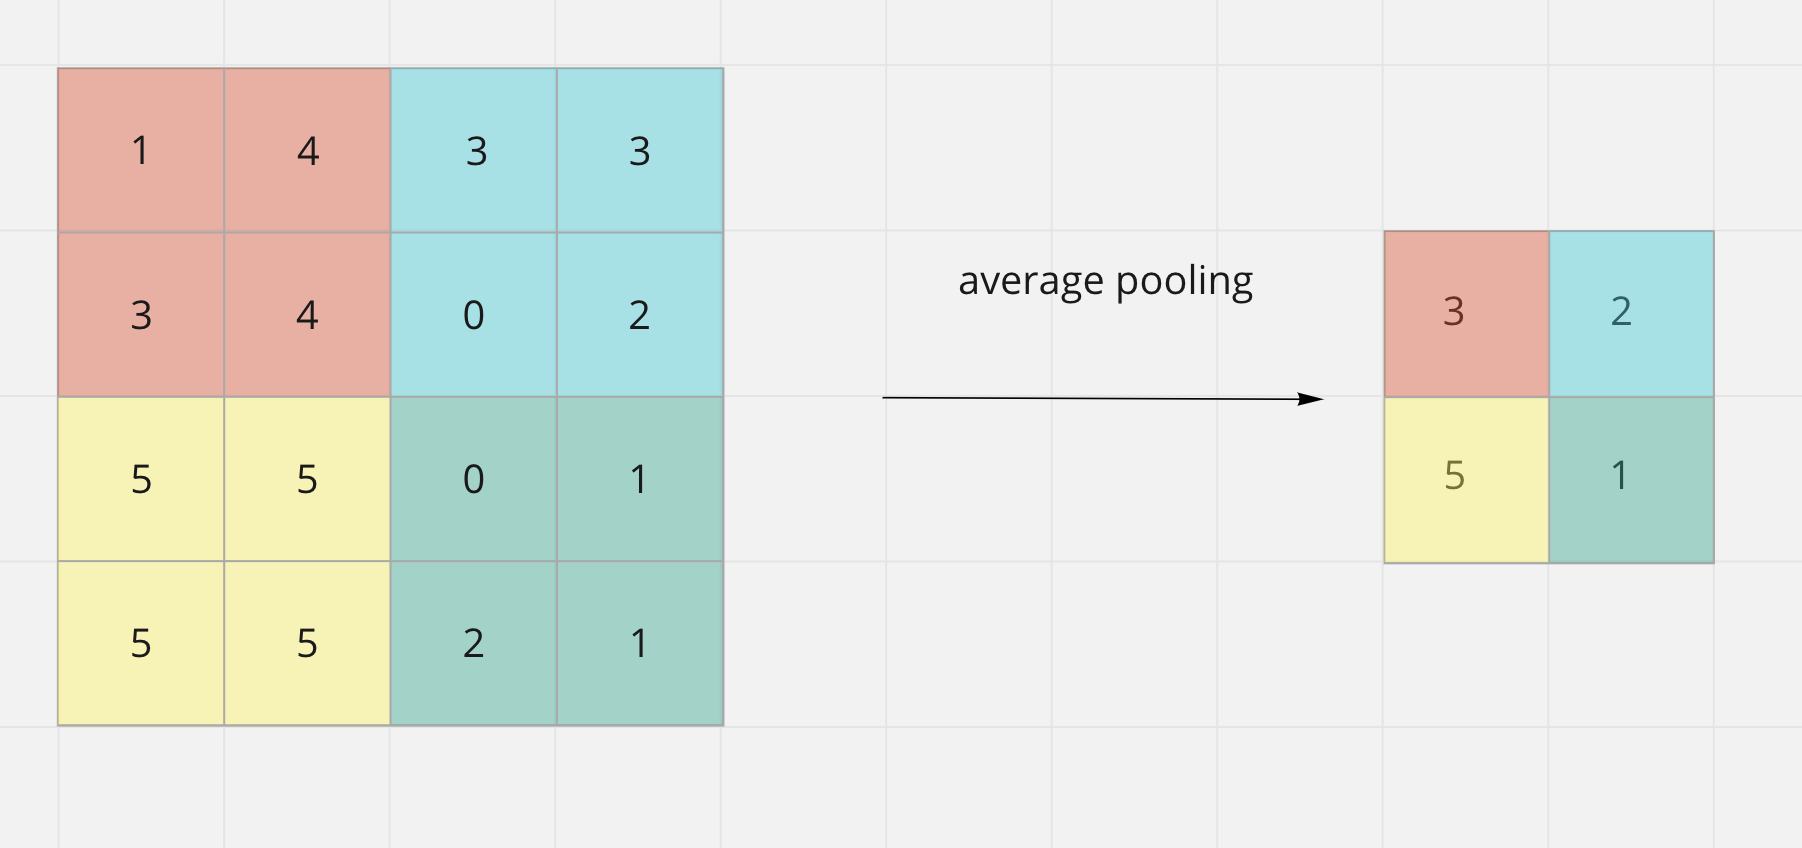
\includegraphics[scale=0.3]{images/2d_pooling.png}
\end{center}
В случае пуллинга латентных пространств мы будем использовать 3d пуллинги вместа 2d пуллингов, если новая размерность нам будет не подходить из-за все еще большого количества исходов. Соответственно в случае 3d пуллинга могут возникнуть проблемы, что пуллинг будет проходить межлу различными каналами, кторые могут быть не связаны между собой. В таком случае мы будем использовать 2d пуллинги с большим окном. \\
Пример 3d пуллинга:
\begin{center}
    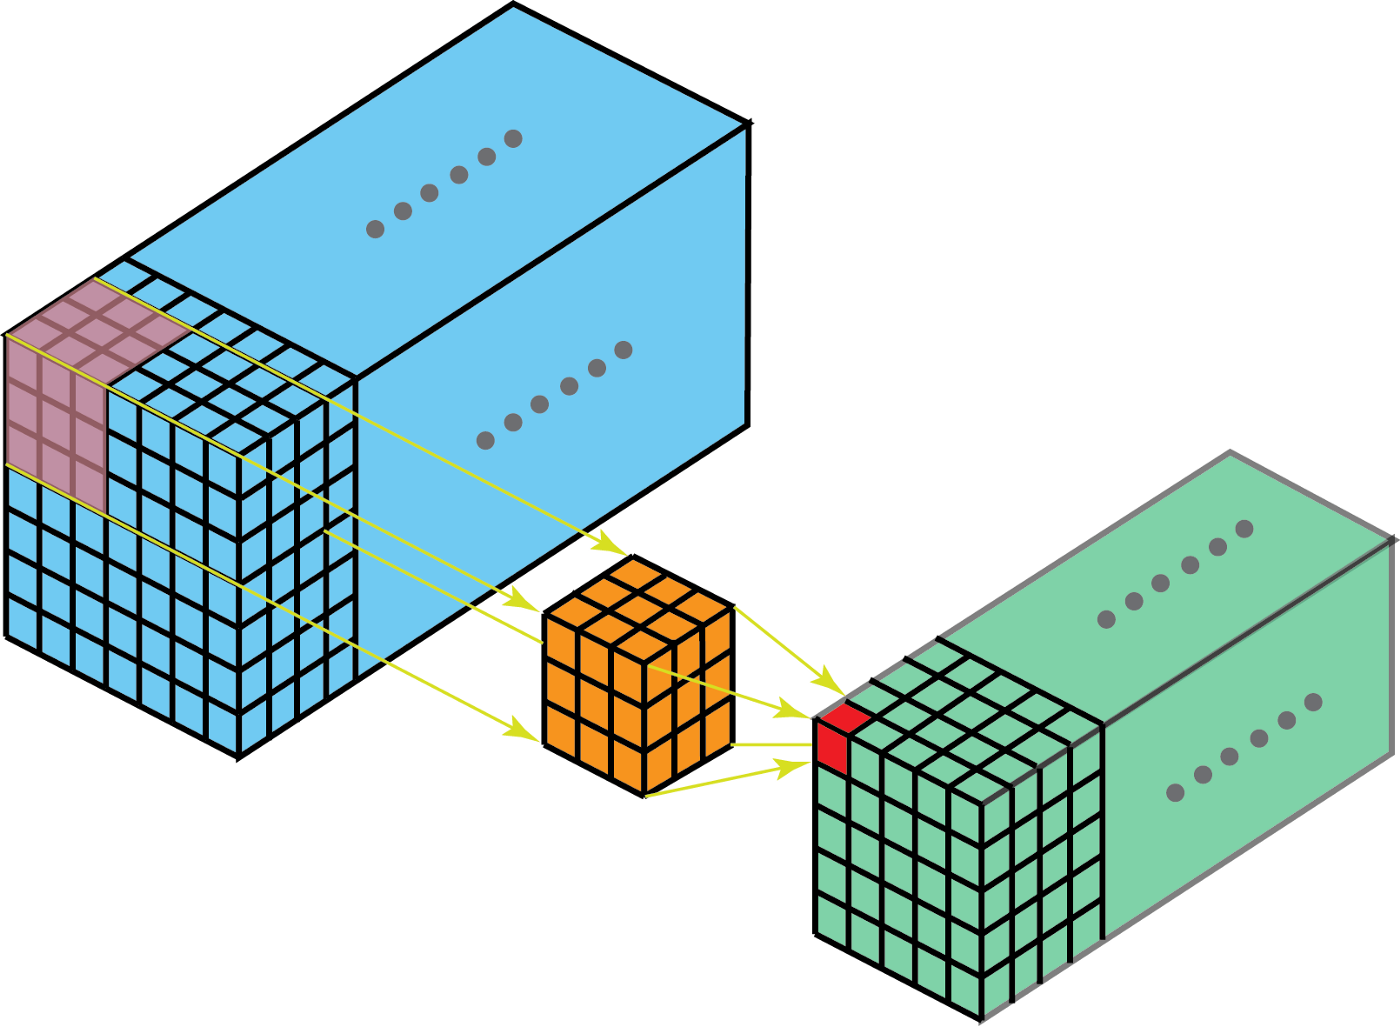
\includegraphics[scale=0.3]{images/3d_pooling.png}
\end{center}
% https://towardsdatascience.com/types-of-convolution-kernels-simplified-f040cb307c37
 
\newpage
\section{Трансформация пространства}
Рассмотрим подробнее каждое из пространств и подумаем как именно можно их сужать и какие гиперпараметры могут быть. Здесь мы рассотрим это с логической точки зрения, качетсвенно на практике мы рассмотрим в следующем параграфе
\subsection{Входное пространство}
Рассмотрим более подробно сужение на входном простратсве, насколько мы знаем $X$ представляет собой тензор размера (28, 28). При использовании дискретизации на 2 значения (0, 1) полученное простраство имеет размер $2^{28 * 28}$, что очень много, поэтому перед дискретизацией мы будем использовать пуллинги. Рассмотрим примеры входных пространств:
\begin{center}
    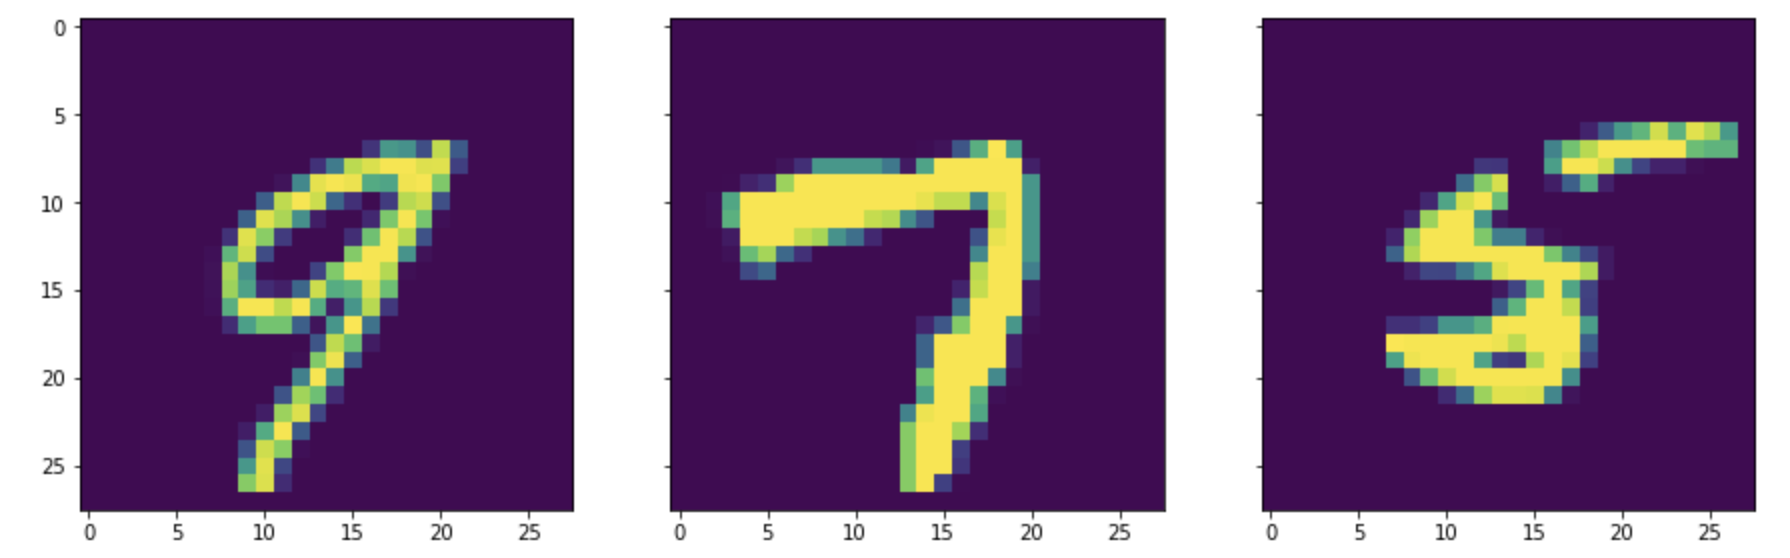
\includegraphics[scale=0.5]{images/plt_input.png}
\end{center}
Как видно картинки представляют собой узкие линии значений близких к 1. Соответственно градиент по картинке высокий. Соответственно при использовании усреднения картинка получится размытая и не будет обладать большим количеством информации о том, что было изначально нарисовано на картинке. \\
Пример использования $Average Pooling$ с окном (7, 7) c навешенной дискретизацией  $discrete$:
\begin{gather}
\begin{aligned}  
discrete(x) = 
\begin{cases}
    0, & \text{if } x\leqslant 0.5\\
    1,              & \text{otherwise}
\end{cases}
\end{aligned}
\end{gather}
\begin{center}
    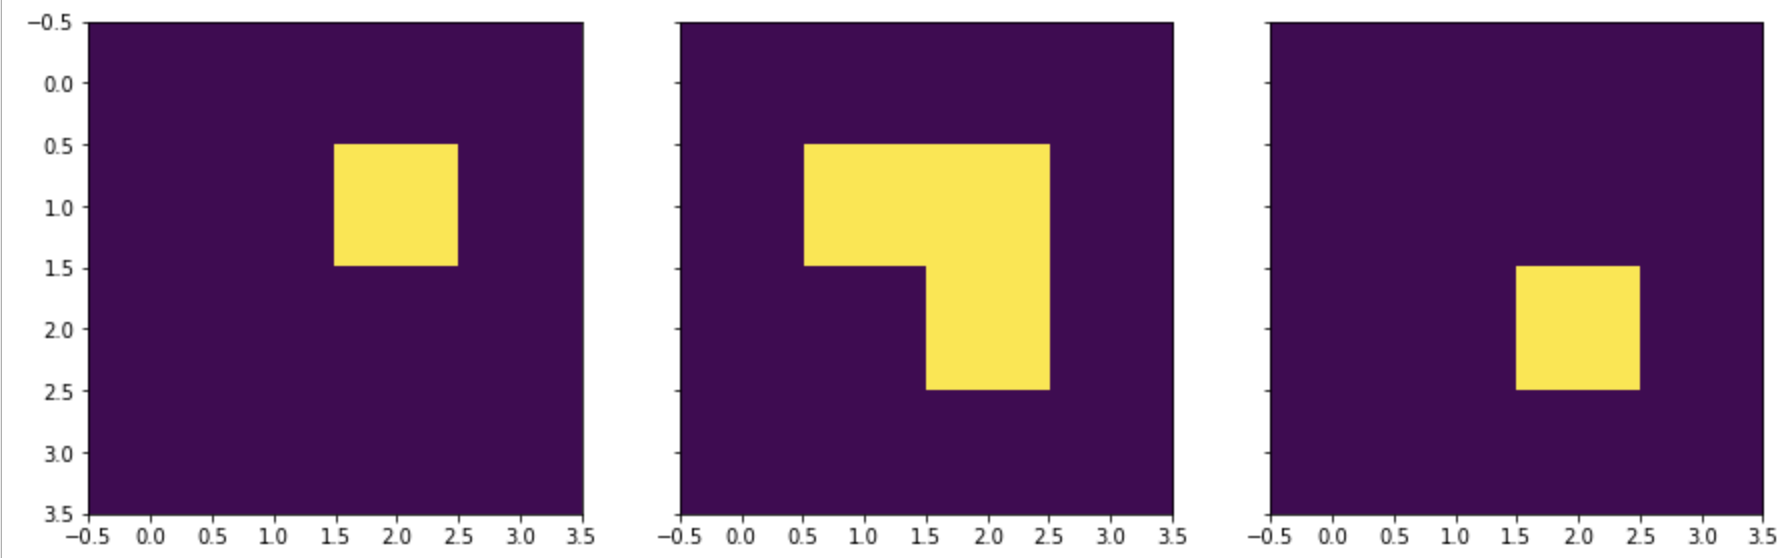
\includegraphics[scale=0.5]{images/plt_arg_7.png}
\end{center}
Праклика показывает что полученное представление не переносит много информации с входного пространства. Если выбирать в окне максимум полученное изображение не будет размываться, а значит будет сохранятся больше информации. \\
Пример использования $Max Pooling$ с окном (7, 7) c навешенной дискретизацией  $discrete$:
\begin{center}
    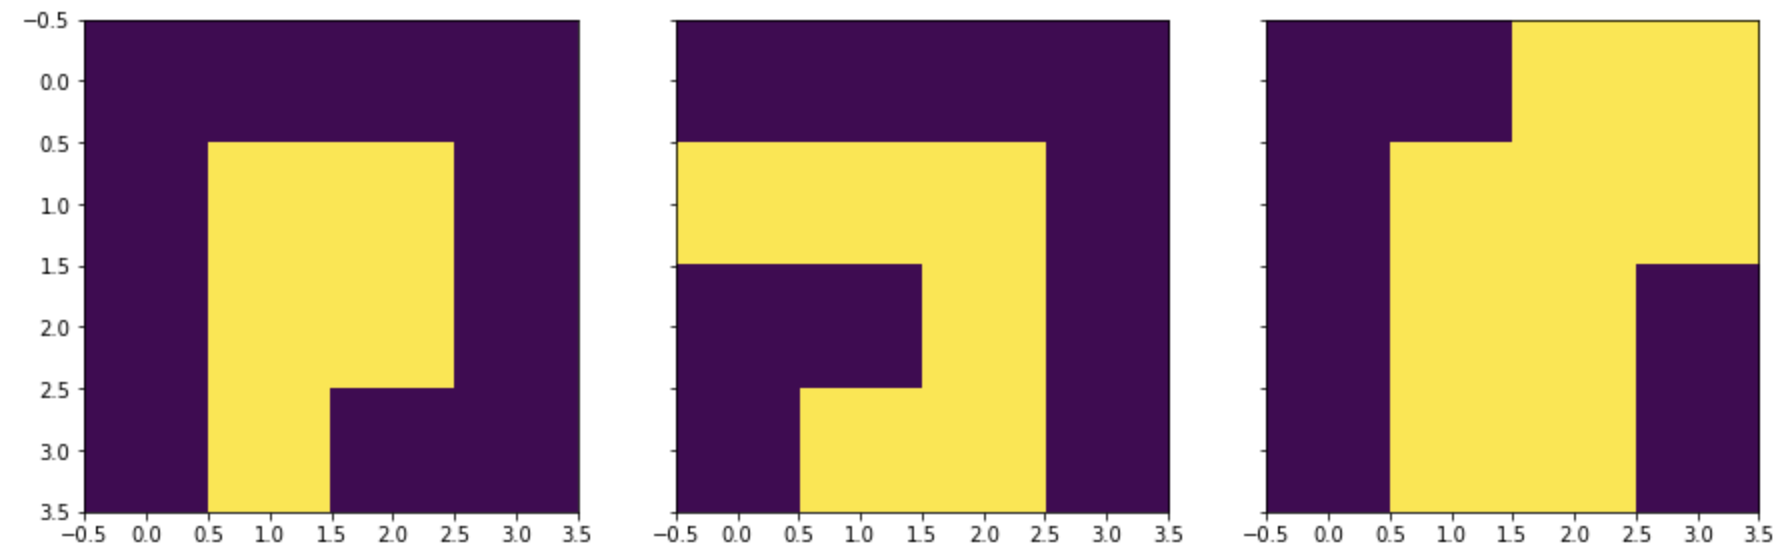
\includegraphics[scale=0.5]{images/plt_max_7.png}
\end{center}
В качетстве увеличения информации имеет смысл уменьшить окно пуллинга. При этом пространство будет больше и больше вероятность инъективности отображения, но количество перетекаемой информации также увеличится. \\
Пример использования $Max Pooling$ с окном (4, 4) c навешенной дискретизацией  $discrete$:
\begin{center}
    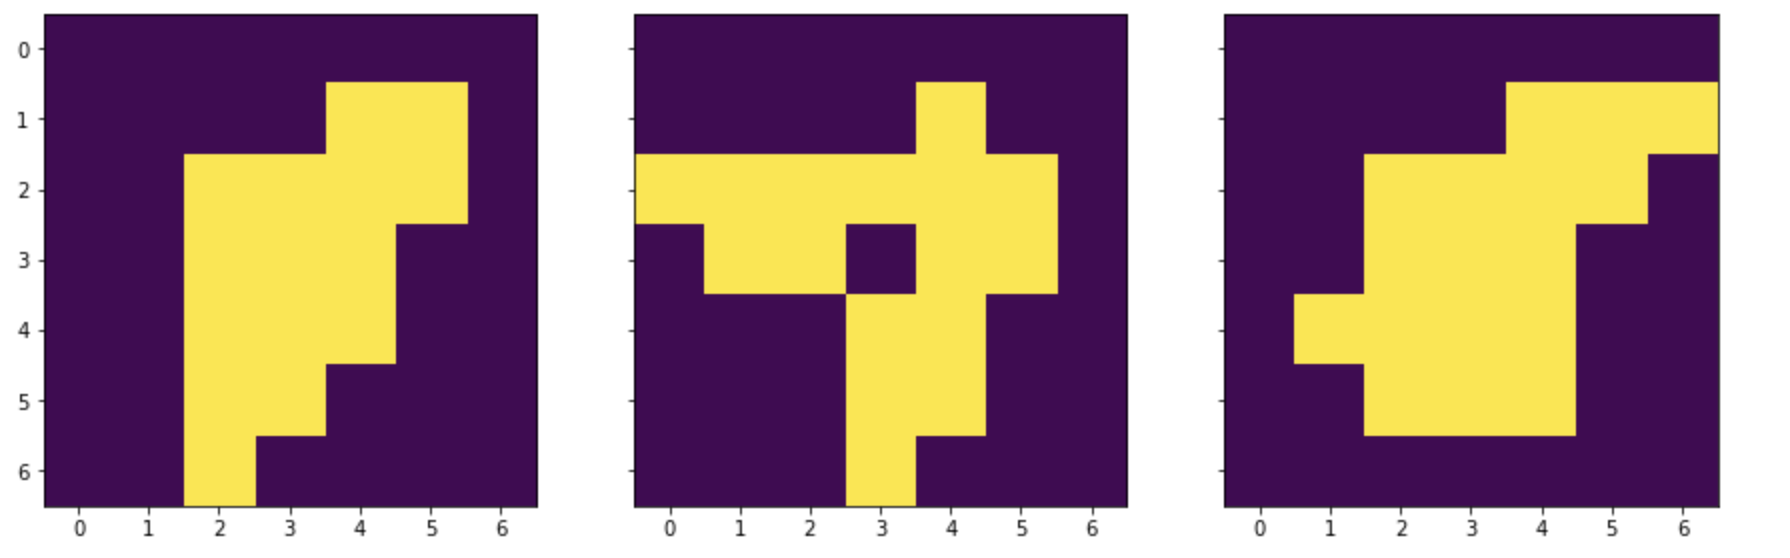
\includegraphics[scale=0.5]{images/plt_max_4.png}
\end{center}

\subsection{Латентное финальное простраство}
Здесь мы рассотрим пространство $Z_3$ которое является выходным слоем сети. Во время обучения от данного слоя берется функция $Softmax$ и уже сравнивается с $one hot$ векторов метки изобажения. Соответственно в пространстве $Z_3$ нам не важны сами значения, нам важен их порядок и индекс наибольшего значения, так как после применения операции $Softmax$ наибольшее значение из всех станет близки к 1, а все остальные близки к 0
\begin{gather}
\begin{aligned}  
softmax(x_i) \approx 
\begin{cases}
    1, & \text{if } i = max\_index\\
    0, & \text{if } i \neq max\_index
\end{cases}
\end{aligned}
\end{gather}
Поэтому нам не так важно распеделение на финальном слое, как важен порядок. Поэтому преобразование на финальном латентном пространстве будет функция $Softmax$.
\subsection{Промежуточные латентные пространства}
В качетсве примера возьмем устройство пространства $Z_1$, пространство $Z_2$ устроено аналогично, так как оно получается таким же образом, а имеено с помощью сверточного слоя. Напомним что пространство $Z_1$ имеет размерность $(dataset\_size, 16, 14, 14)$ \\
В качестве примера рассмотрим выход $z_1 \in Z_1$ - а именно результат свертки одной из входных картинок. Разложим тензор по всем 16 каналов: 
\begin{center}
    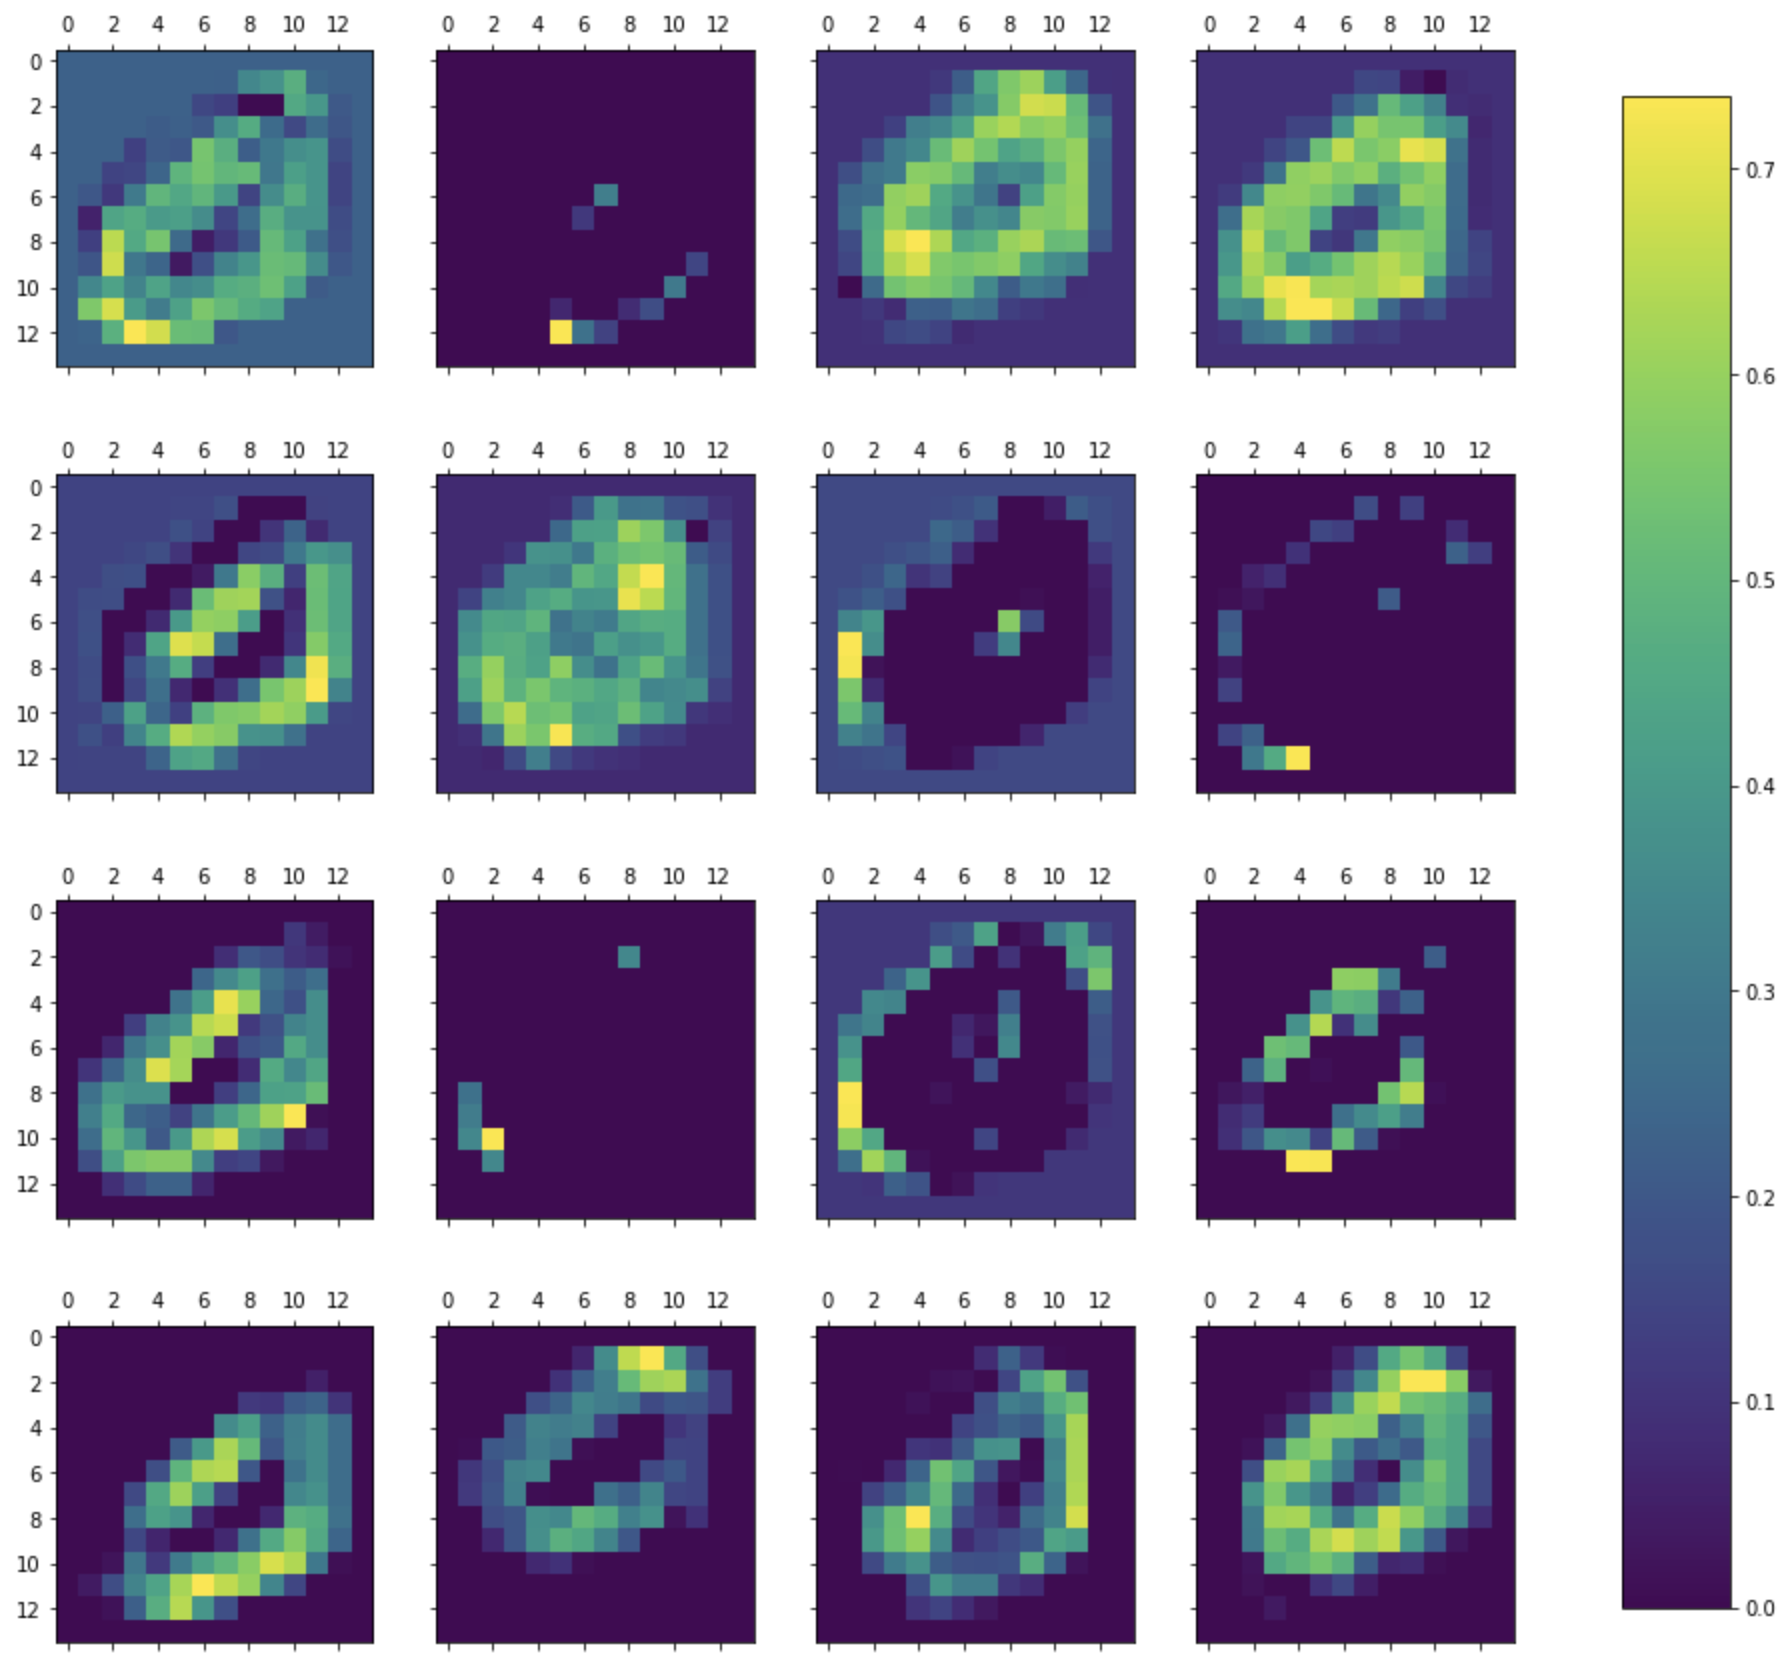
\includegraphics[scale=0.5]{images/plt_z1.png}
\end{center}
Как видно, каждый из 16ти различных каналов представляет собой такое же изображение, где каждая ячейка показывает как реагирует соответствующее окно на определенный фильтр, который сответствует данному каналу. С точки зрения информации нам важно какие места реагируют на различные свертки-фильтры, то есть нам важно понимать как утроены большие значения по признакам (зеленые, желтые на картинке). \\
Для дальнейшей дискретизации нам важно как распределены значения в пространстве по каждому призраку. Для этого посчитаем 0.01 квантиль ($min\_hidden\_border$) и 0.99 квантиль ($max\_hidden\_border$) для каждого из признаков по выборке:
\begin{center}
    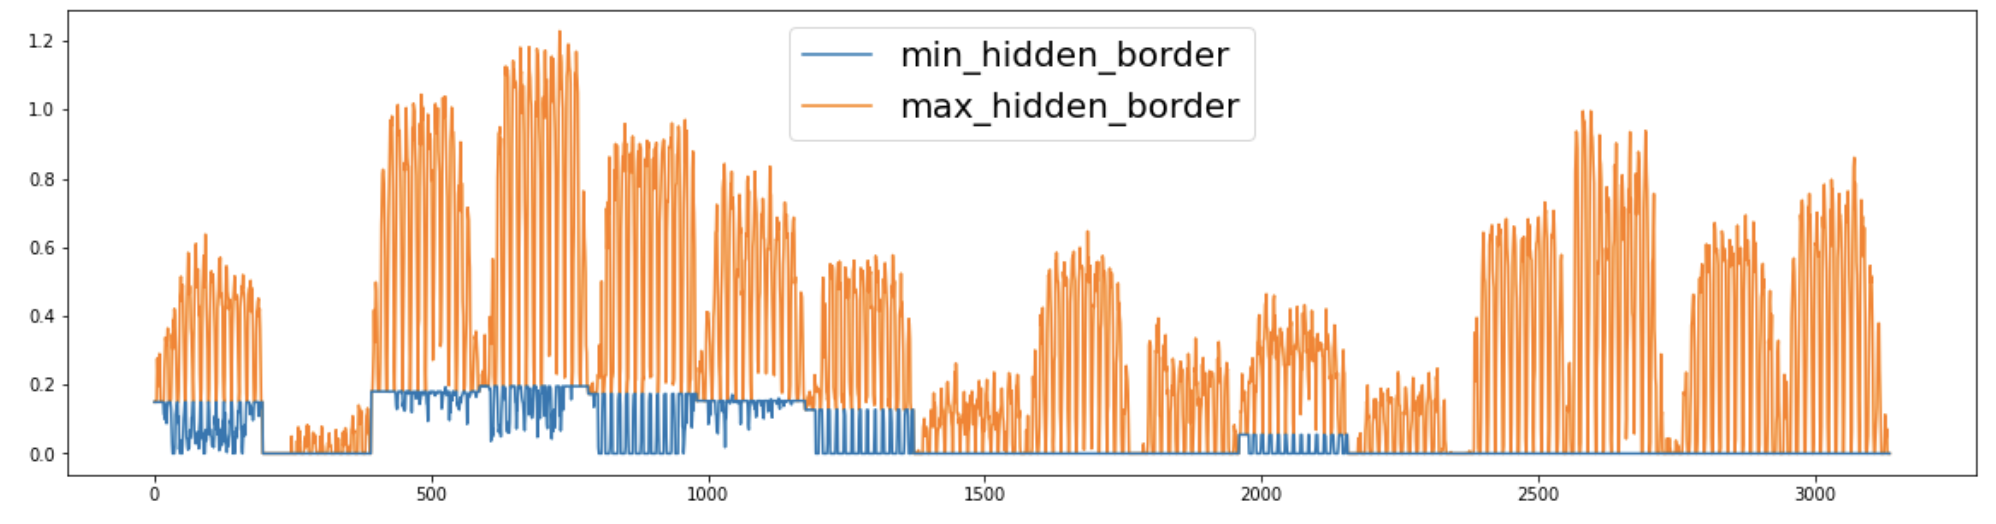
\includegraphics[scale=0.5]{images/z1_borders.png}
\end{center}
Также посчитаем среднее $hidden\_mean$ и дисперсию $hidden\_std$ по каждому признаку:
\begin{center}
    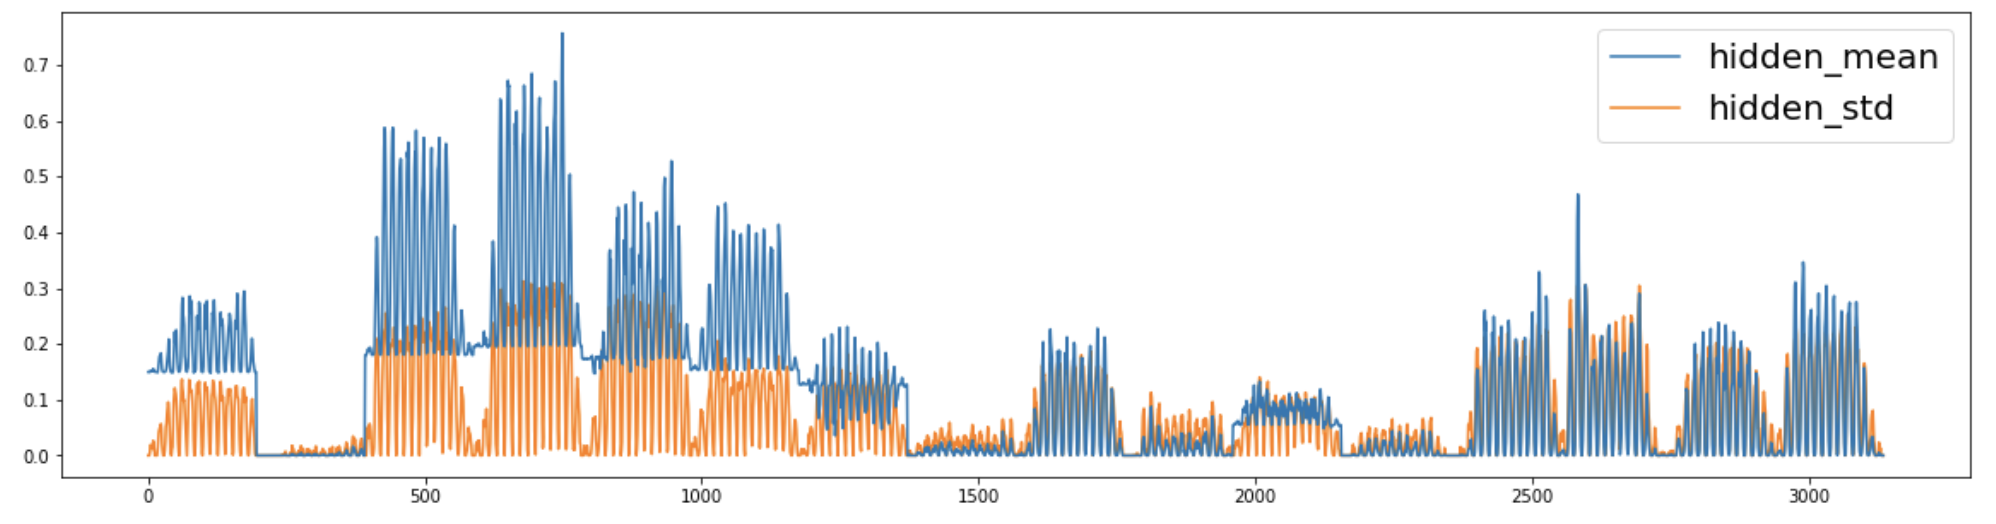
\includegraphics[scale=0.5]{images/z1_means.png}
\end{center}
Как видно распределение по каждому призаку отличаются, отсюда можно сделать вывод что при дискретизации значения к которым будут приближаться пространства будут для каждого признака различны и расчитываться из соответствующих для них $min\_hidden\_border$ и $max\_hidden\_border$. \\
Поскольку нам важно понимать как утроены места с большими значениями в качестве пуллинга будет использоваться $maxpool$, поскольку $avgpool$ будет делать значения более размытыми. Пример дискретизации с последовательным применением пуллинга и дискретизации, то есть дискретизация проводится по уже сжатой выборке:
\begin{center}
    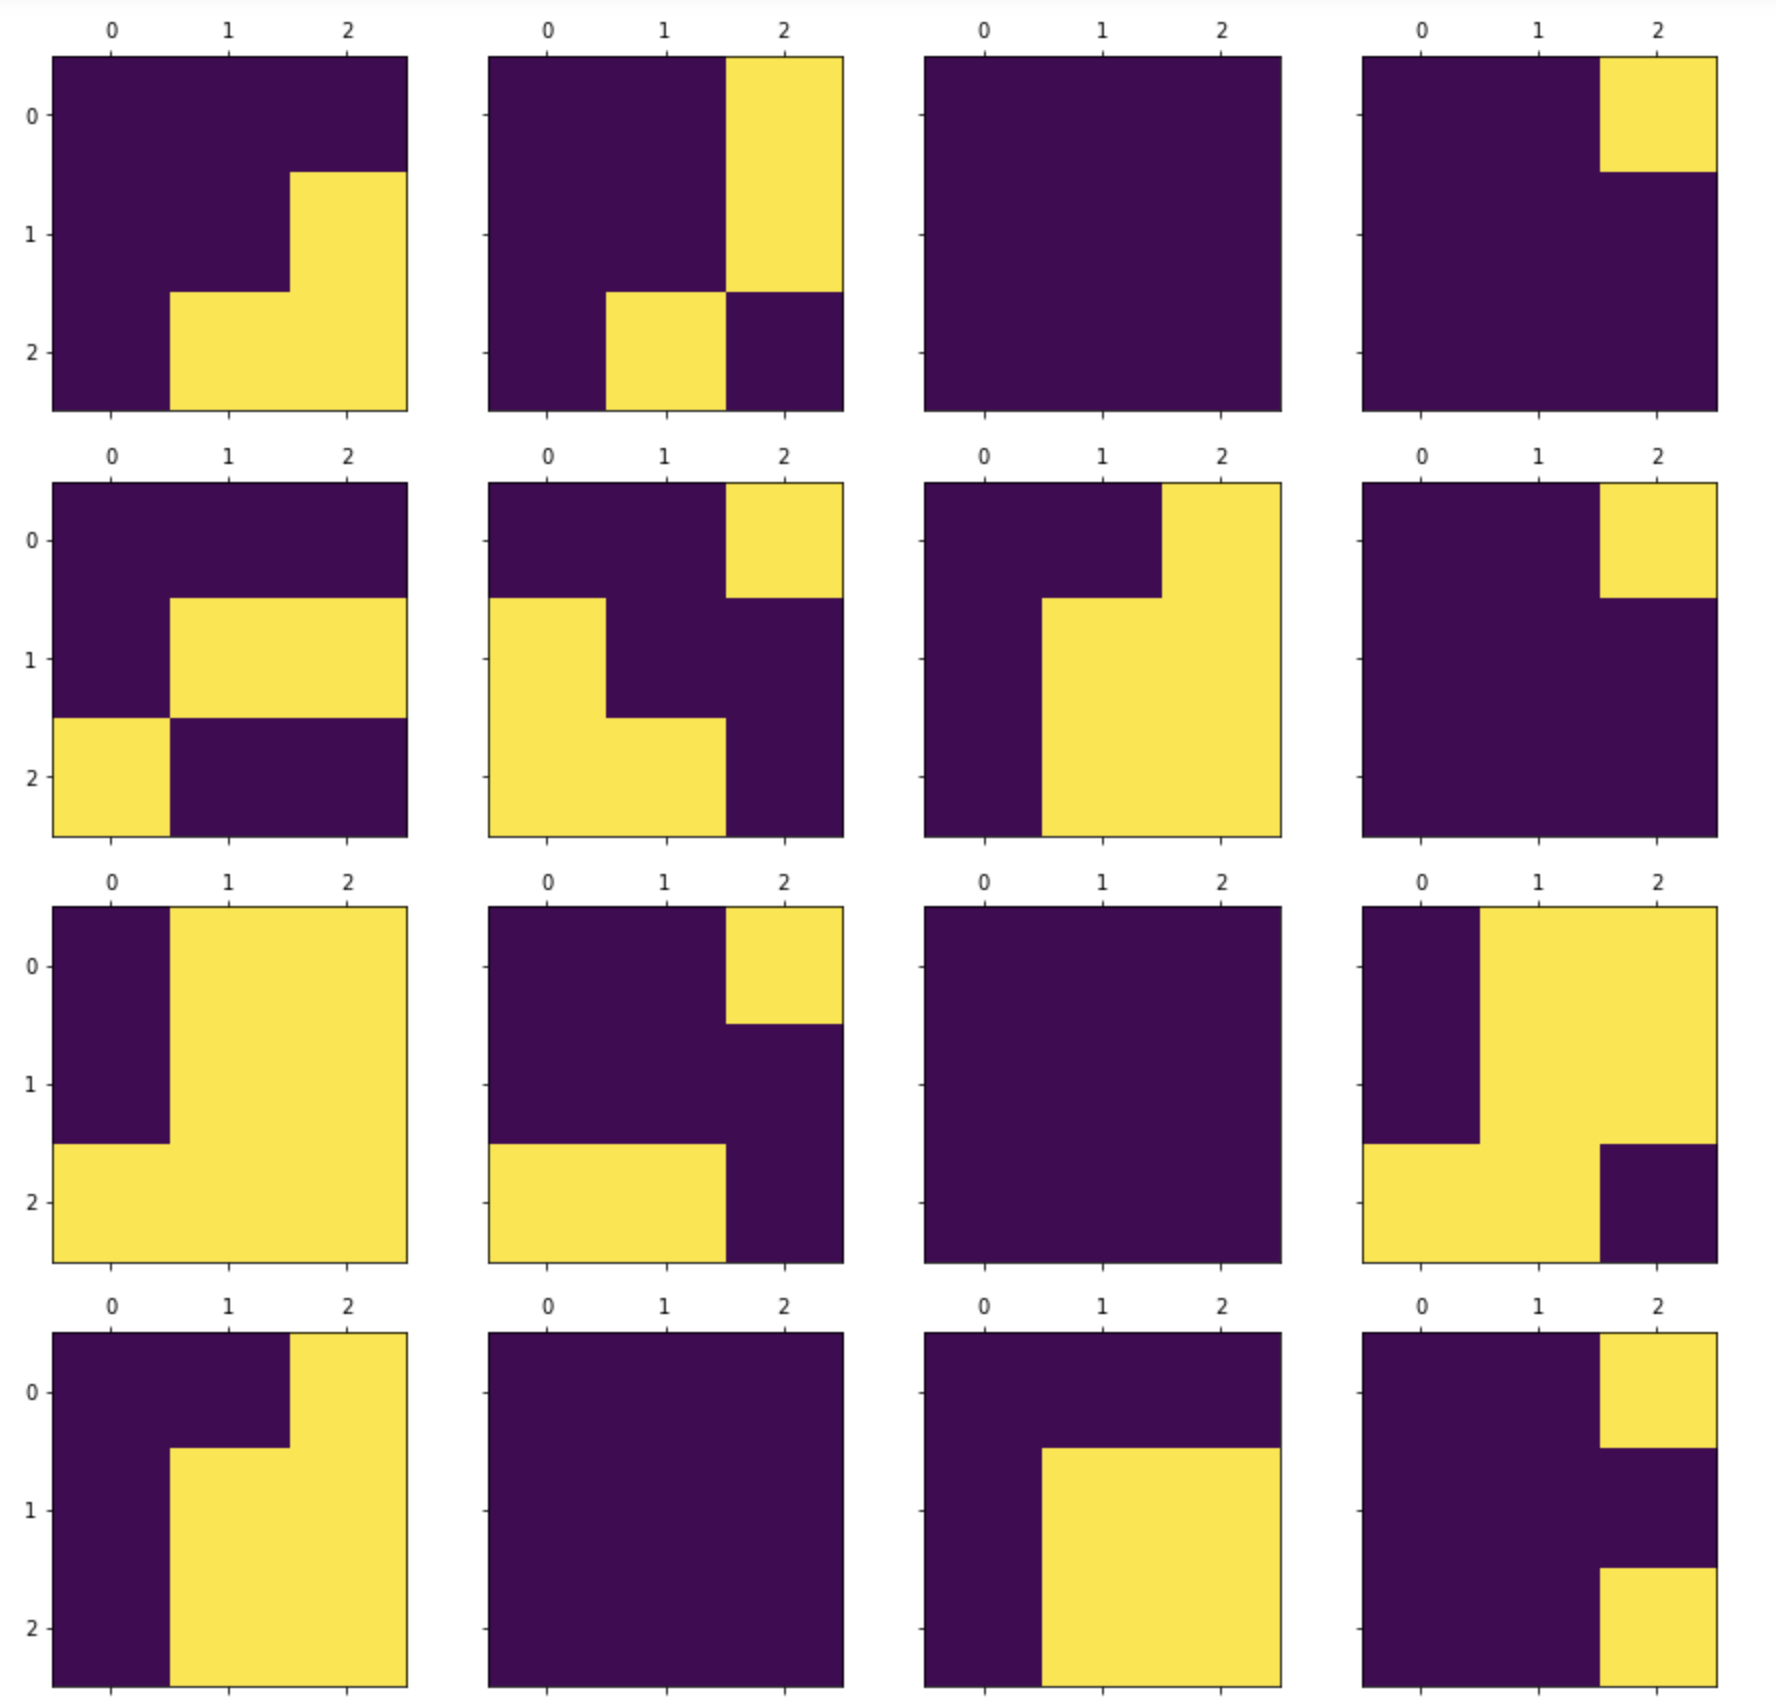
\includegraphics[scale=0.5]{images/z1_max_7.png}
\end{center}\
Аналогичную операцию сужения пространства будем проводить с следующем латентным пространством $Z_2$. Параметры пуллинга остаются гиперпараметрами и устанавливаются на валидации. При этом условие проводить $MaxPool2d$ или $MaxPool3d$ также остается гиперпараметром, так как каналы более независимы друг от друга чем значения внутри каждого канала. Но при этом при смешиваниии каналов дискретизация приводит к меньшему простанству и уменьшается риск инъективности отобрания. 





\newpage
\section{Информационные метрики}
\subsection{Случай без сужения пространства}
Для оценки метрики 
\begin{gather}
\begin{aligned}
min_{Z} I[X, Z] - \beta * I[Z, Y]
\end{aligned}
\end{gather} 
требуется считать совместные информационные эвристики между латентным пространством и входным/выходным, вспомим формулу информации между латентным пространством $Z$ и входным пространством $X$
\begin{gather}
\begin{aligned}
    I[X, Z] = - \EX_{p(x, z)}\log(\frac{p(x)p(z)}{p(x, z)}) = \\ \sum_{i=0}^{len\_dataset}p_{XZ}(x=x_i, z=z_i) * \log(\frac{p_{XZ}(x=x_i, z=z_i)}{p_X(x=x_i) * p_Z(z=z_i)})
\end{aligned}
\end{gather}    
где 
\begin{gather}
\begin{aligned}
p_X(x=x_i) = count(discrite(x_i)) / len(dataset) \\
p_Z(z=z_i) = count(discrite(z_i)) / len(dataset) \\
p_{XZ}(x=x_i, z=z_i) = count(concat(discrite(x_i), discrite(z_i))) / len(dataset) 
\end{aligned}
\end{gather}
То есть мы считаем количество элементов эдементов в датасете которые перешли в одни и те же дискретные исходы и на основе этих количеств строим вероятностное пространство. Заметим что свойства вероятностной меры соблюдены: сумма всеъ вероятностей равна 1, мера не отрицательна, соблюдедается аддитивность. \\
Аналогично считается $I[Y, Z]$:
\begin{gather}
\begin{aligned}
    I[Y, Z] = - \EX_{p(y, z)}\log(\frac{p(y)p(z)}{p(y, z)}) = \\ \sum_{i=0}^{len\_dataset}p_{YZ}(y=y_i, z=z_i) * \log(\frac{p_{YZ}(y=x_i, z=z_i)}{p_Y(y=y_i) * p_Z(z=z_i)})
\end{aligned}
\end{gather} 
только при этом не происходит дискретизация для $Y$, тк оно и так принимает целые значения от 0 до 9. \\
Соответственно если рассматривать пространства $p_{XZ}, p_{YZ}, p_{X}, p_{Z}$ без сужения велика вероятность получения равномерного распределения независимо от латентного пространства, то есть 
\begin{gather}
\begin{aligned}
p_X(x=x_i) = \frac{count(discrite(x_i))}{len(dataset)} \approx \frac{1}{len(dataset)} \\
p_Z(z=z_i) = \frac{count(discrite(z_i))}{len(dataset)} \approx \frac{1}{len(dataset)} \\
p_{XZ}(x=x_i, z=z_i) = \frac{count(concat(discrite(x_i), discrite(z_i)))}{len(dataset) } \approx \frac{1}{len(dataset)} 
\end{aligned}
\end{gather}
Это будет для больших пространств пространств, таких как входной слой или первые слои свертки, где также много параметров. Дело в том, что дискретизация в таких случаях будет инъективным отображением как на входном пространстве, так и на латентном, также функция преобразования (часть forward pass) будет инъективной, а значит выполняются такие апроксимации для любых латентных пространств независимо от эпохи обучения. Соответветственно информация будет константной и не будет менятся от эпохи обучения, как и метрика Information Bottleneck (15). \\
Соответственно для решения этого нам потребуются уменьшение вероятностных пространств, чтобы избавится от инвариантоности и сделать распределение неравномерным. Также без сужение пространства построение вероятностного пространства и подсчет информационных метрик ресурсно затратно, так как требуется хранить большой сет и итерироваться по нему, что долго. \\
Представим инфмаорционные метрики на графиках в зависимости от эпохи обучения. Всего было 10 эпох обучения, в каждой из итераций строилось новое вероятностное пространство и по нему считались давнные эвристики.
\begin{center}
    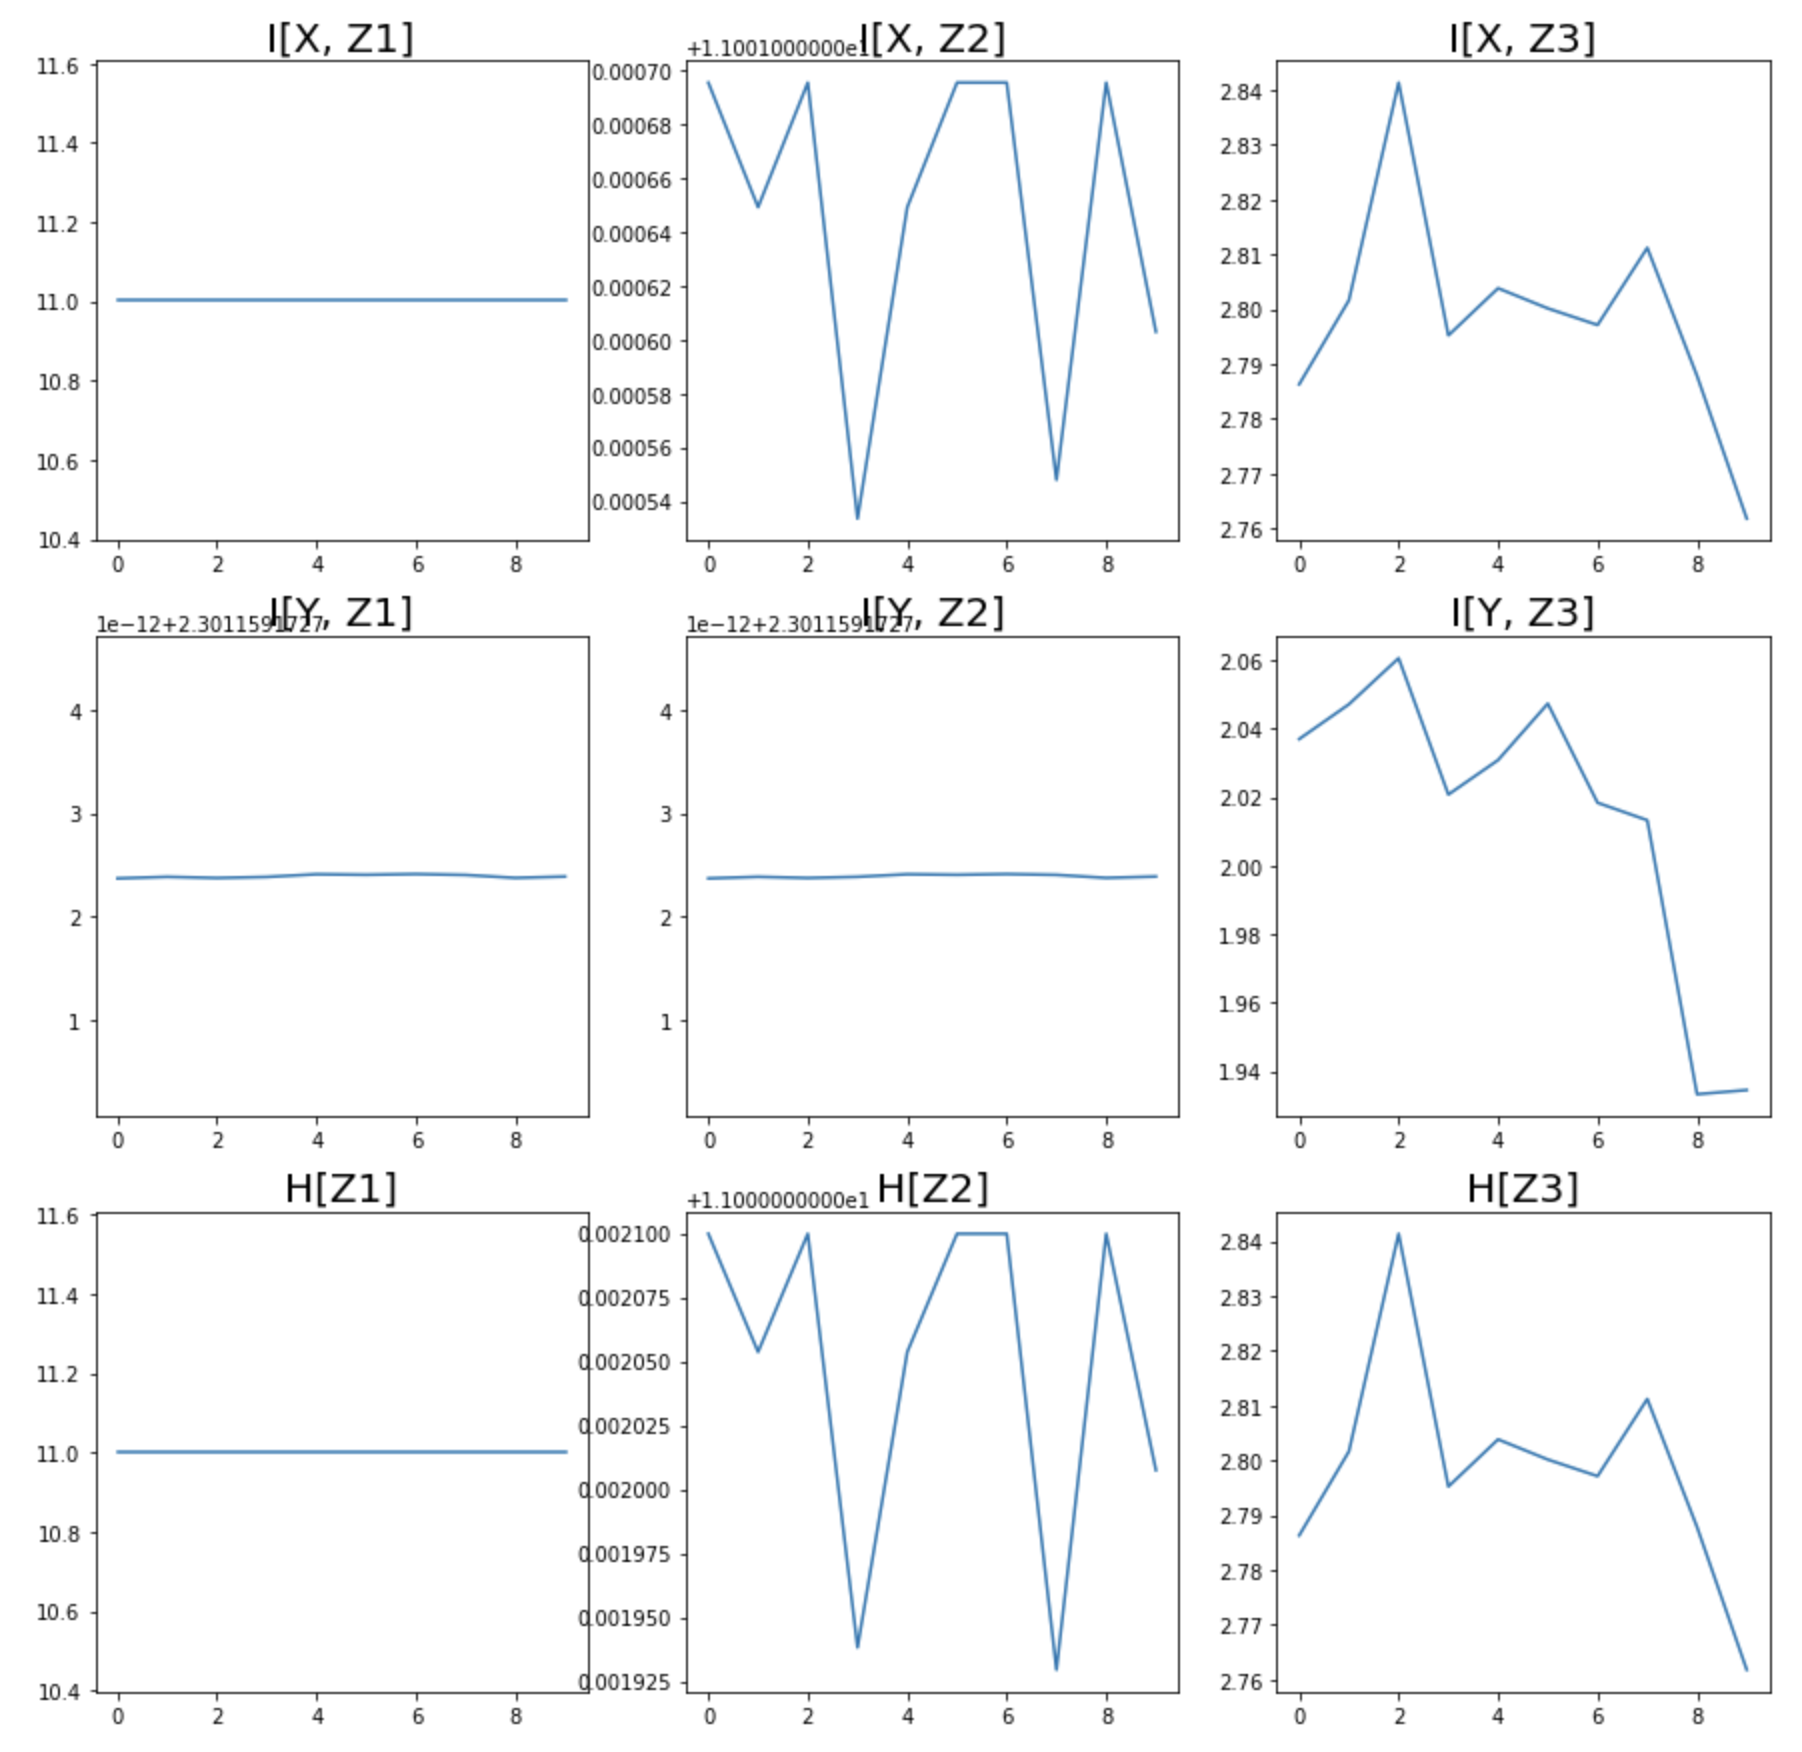
\includegraphics[scale=0.45]{images/inf_without_comp.png}
\end{center}
Как можно заметить $H[Z_1], I[X, Z_1], I[Y,Z_1]$ статичны независимо от эпохи. Это происходит из-за того что построенные вероятностные пространства распределены равномерно, это еще раз подтверждает то, что латентное пространство требуется сужать. Также метрики не имею никакую тенденцию. Мы пришли к выводу что задача нейронной сети уменьшение эвристики: 
\begin{gather}
\begin{aligned}
I[X, Z] - \beta * I[Z, Y]
\end{aligned}
\end{gather}
Здесь же не наблюдается уменьшение метрики $I[X, Z]$ и увеличение метрики $I[Y, Z]$ ни для ни одного латентного пространства $Z_1, Z_2, Z_3$.
\subsection{Случай сужения пространства}
Рассмотрим пример с сужением вероятностных пространств и посчитаем на них аналогично информационные эвристики в зависимости от эпохи:
\begin{center}
    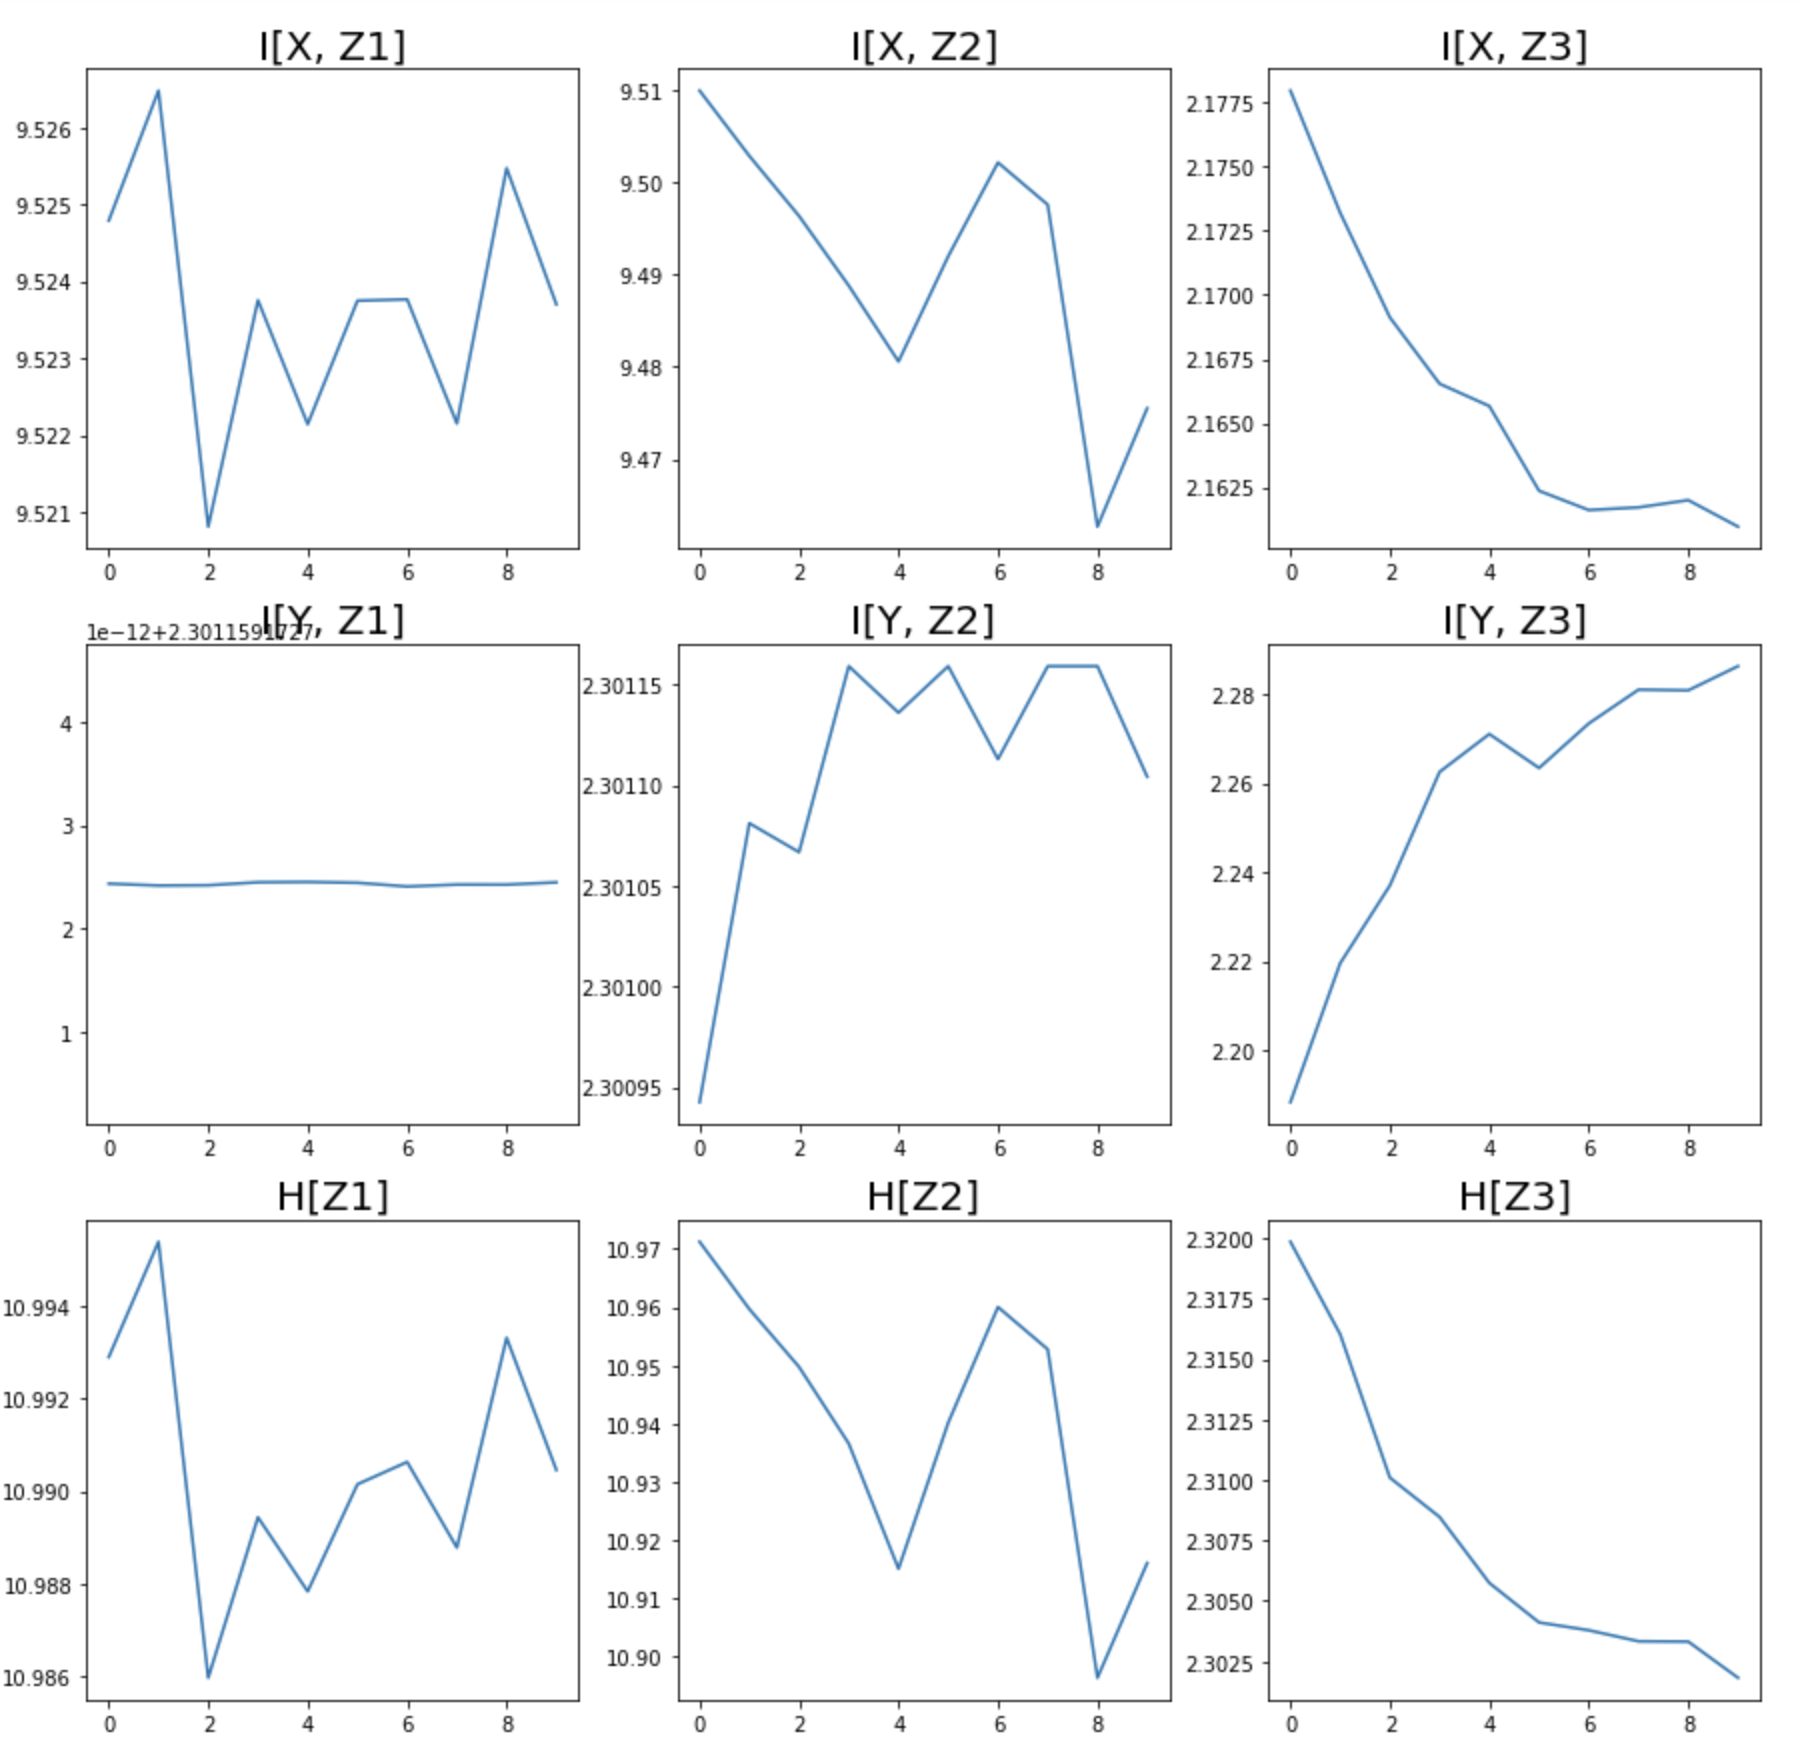
\includegraphics[scale=0.5]{images/inf_comp_v1.png}
\end{center} 

Здесь в данном примере в качестве гиперпараметров возьмем:
\begin{enumerate}
\item $waist\_input = MaxPool2d((4, 4))(input)$
\item $waist\_z1 = MaxPool3d((1, 4, 4))(z1)$
\item $waist\_z2 = MaxPool3d((1, 3, 3))(z2)$
\item $waist\_z3 = Softmax(z3)$
\end{enumerate}
То есть в промежуточных латентных слоях не смешивались каналы между собой. \\
Здесь проще всего рассмотреть как ведут себя информация между входным пространством и латентным $I[X, Z]$ и энтропия латентных пространств $H[Z]$. Как видно на графике данные эвристики уменьшаюся по мере обучения, причем чем проще латентное пространство устроено тем более функция от эпохи монотонная. Например $I[X, Z_3]$ и $H[Z_3]$ имеют более выраженое уменьшение с увеличением эпохи чем аналогичные эвристики только для $Z_2$ и $Z_1$. Аналогичное можно сказать про информацию между выходом и латентными пространствами $I[Y, Z]$. Чем больше $Z_i$ тем более монотона устроена функция. Только при этом $I[X, Z$ уменьшается в то время как $I[Y, Z]$ увеличивается. Более выроженная монотонность происходит по причине что пространсво $Z_3$ устроено проще чем другие латентные пространства. $Softmax(z_3)$ стремится к $one\_hot(y)$ для любых соответсвующих $z_3 \in Z_3, & y \in Y$. Таким образом в хорошо обученной сети:
\begin{gather}
\begin{aligned}
I[Y, Z] = \sum_{i=0}^{len\_dataset}p_{YZ}(y=y_i, z=z_i) * \log(\frac{p_{YZ}(y=x_i, z=z_i)}{p_Y(y=y_i) * p_Z(z=z_i)}) \approx \\
\sum_{i=0}^{len\_dataset}p_Y(y=y_i) * \log(\frac{p_Y(y=y_i)}{p_Y(y=y_i) * p_Y(y=y_i)} = \\
- \sum_{i=0}^{len\_dataset}p_Y(y=y_i) * \log(p_Y(y=y_i)) = H(Y) \approx \\
\sum_{i=1}^{10}0.1 * \log(10) = \log(10) \approx 2.3
\end{aligned}
\end{gather}
Как видно в текущем примере $I[Y, Z]$ не достигает максимальной оценки. Увеличение метрики $I[Y, Z]$ и уменьшение метрики $I[X, Z]$ подтвержает нашу гипотезу что метрику Information Bottleneck можно использовать как лосс функции, так как функция $I[X, Z] - \beta * I[Z, Y], \beta > 0$ уменьшается с улучшением сети. При этом информационные метрики для $Z_1$ устроены самым непонятным образом. Это связано с тем что данное латентное пространство наиболее сложное, и в нем наибольшее количество параметров: 
\begin{enumerate}
\item $waist\_input.shape = (1, 7, 7) \Rightarrow len(input\_params) = 2^{1 * 7 * 7} = 2^{49}$
\item $waist\_z1.shape = (16, 3, 3) \Rightarrow len(z1\_params) = 2^{16 * 3 * 3} = 2^{144}$
\item $waist\_z2.shape = (32, 2, 2) \Rightarrow len(z2\_params) = 2^{32 * 2 * 2} = 2^{128}$
\item $waist\_z3.shape = (10) \Rightarrow len(z3\_params) = 2^{10}$
\end{enumerate}
\subsection{Валидация гиперпарметров}
Проведем несколько экспериментов, сравнив информационные метрики для различных вероятностных пространств. Для этого первым экспериментом смешаем каналы для пространств $Z_2$ и $Z_3$, то есть MaxPooling будет проводиться также и по каналам. Этот эксперимент имеет смысл, так как в предъидушем примере латентные пространства имеют слишком большую размерность и как вывод сложные информационные представления. Соответственно смешиваение по каналам позволит уменьшить размерность пространства. В еще одном примере уменьшение размерности пространства будем осуществлять засчет увеличение окна 2d свертк, это позволит не смешивать каналы между собой. Для этого рассмотрим 3 примера с другими сверками. \\
1 пример:
\begin{enumerate}
\item $waist\_input = MaxPool2d((4, 4))(input)$
\item $waist\_z1 = MaxPool3d((2, 4, 4))(z1)$
\item $waist\_z2 = MaxPool3d((2, 3, 3))(z2)$
\item $waist\_z3 = Softmax(z3)$
\end{enumerate}
2 пример:
\begin{enumerate}
\item $waist\_input = MaxPool2d((4, 4))(input)$
\item $waist\_z1 = MaxPool3d((4, 4, 4))(z1)$
\item $waist\_z2 = MaxPool3d((4, 3, 3))(z2)$
\item $waist\_z3 = Softmax(z3)$
\end{enumerate}
3 пример:
\begin{enumerate}
\item $waist\_input = MaxPool2d((4, 4))(input)$
\item $waist\_z1 = MaxPool3d((1, 7, 7))(z1)$
\item $waist\_z2 = MaxPool3d((1, 7, 7))(z2)$
\item $waist\_z3 = Softmax(z3)$
\end{enumerate}
и посчитаем для новых вероятностных пространств информационные метрики.
Примеры 1-3 расположены слева направа на графиках.
\begin{figure}[!htb]
\minipage{0.33\textwidth}
  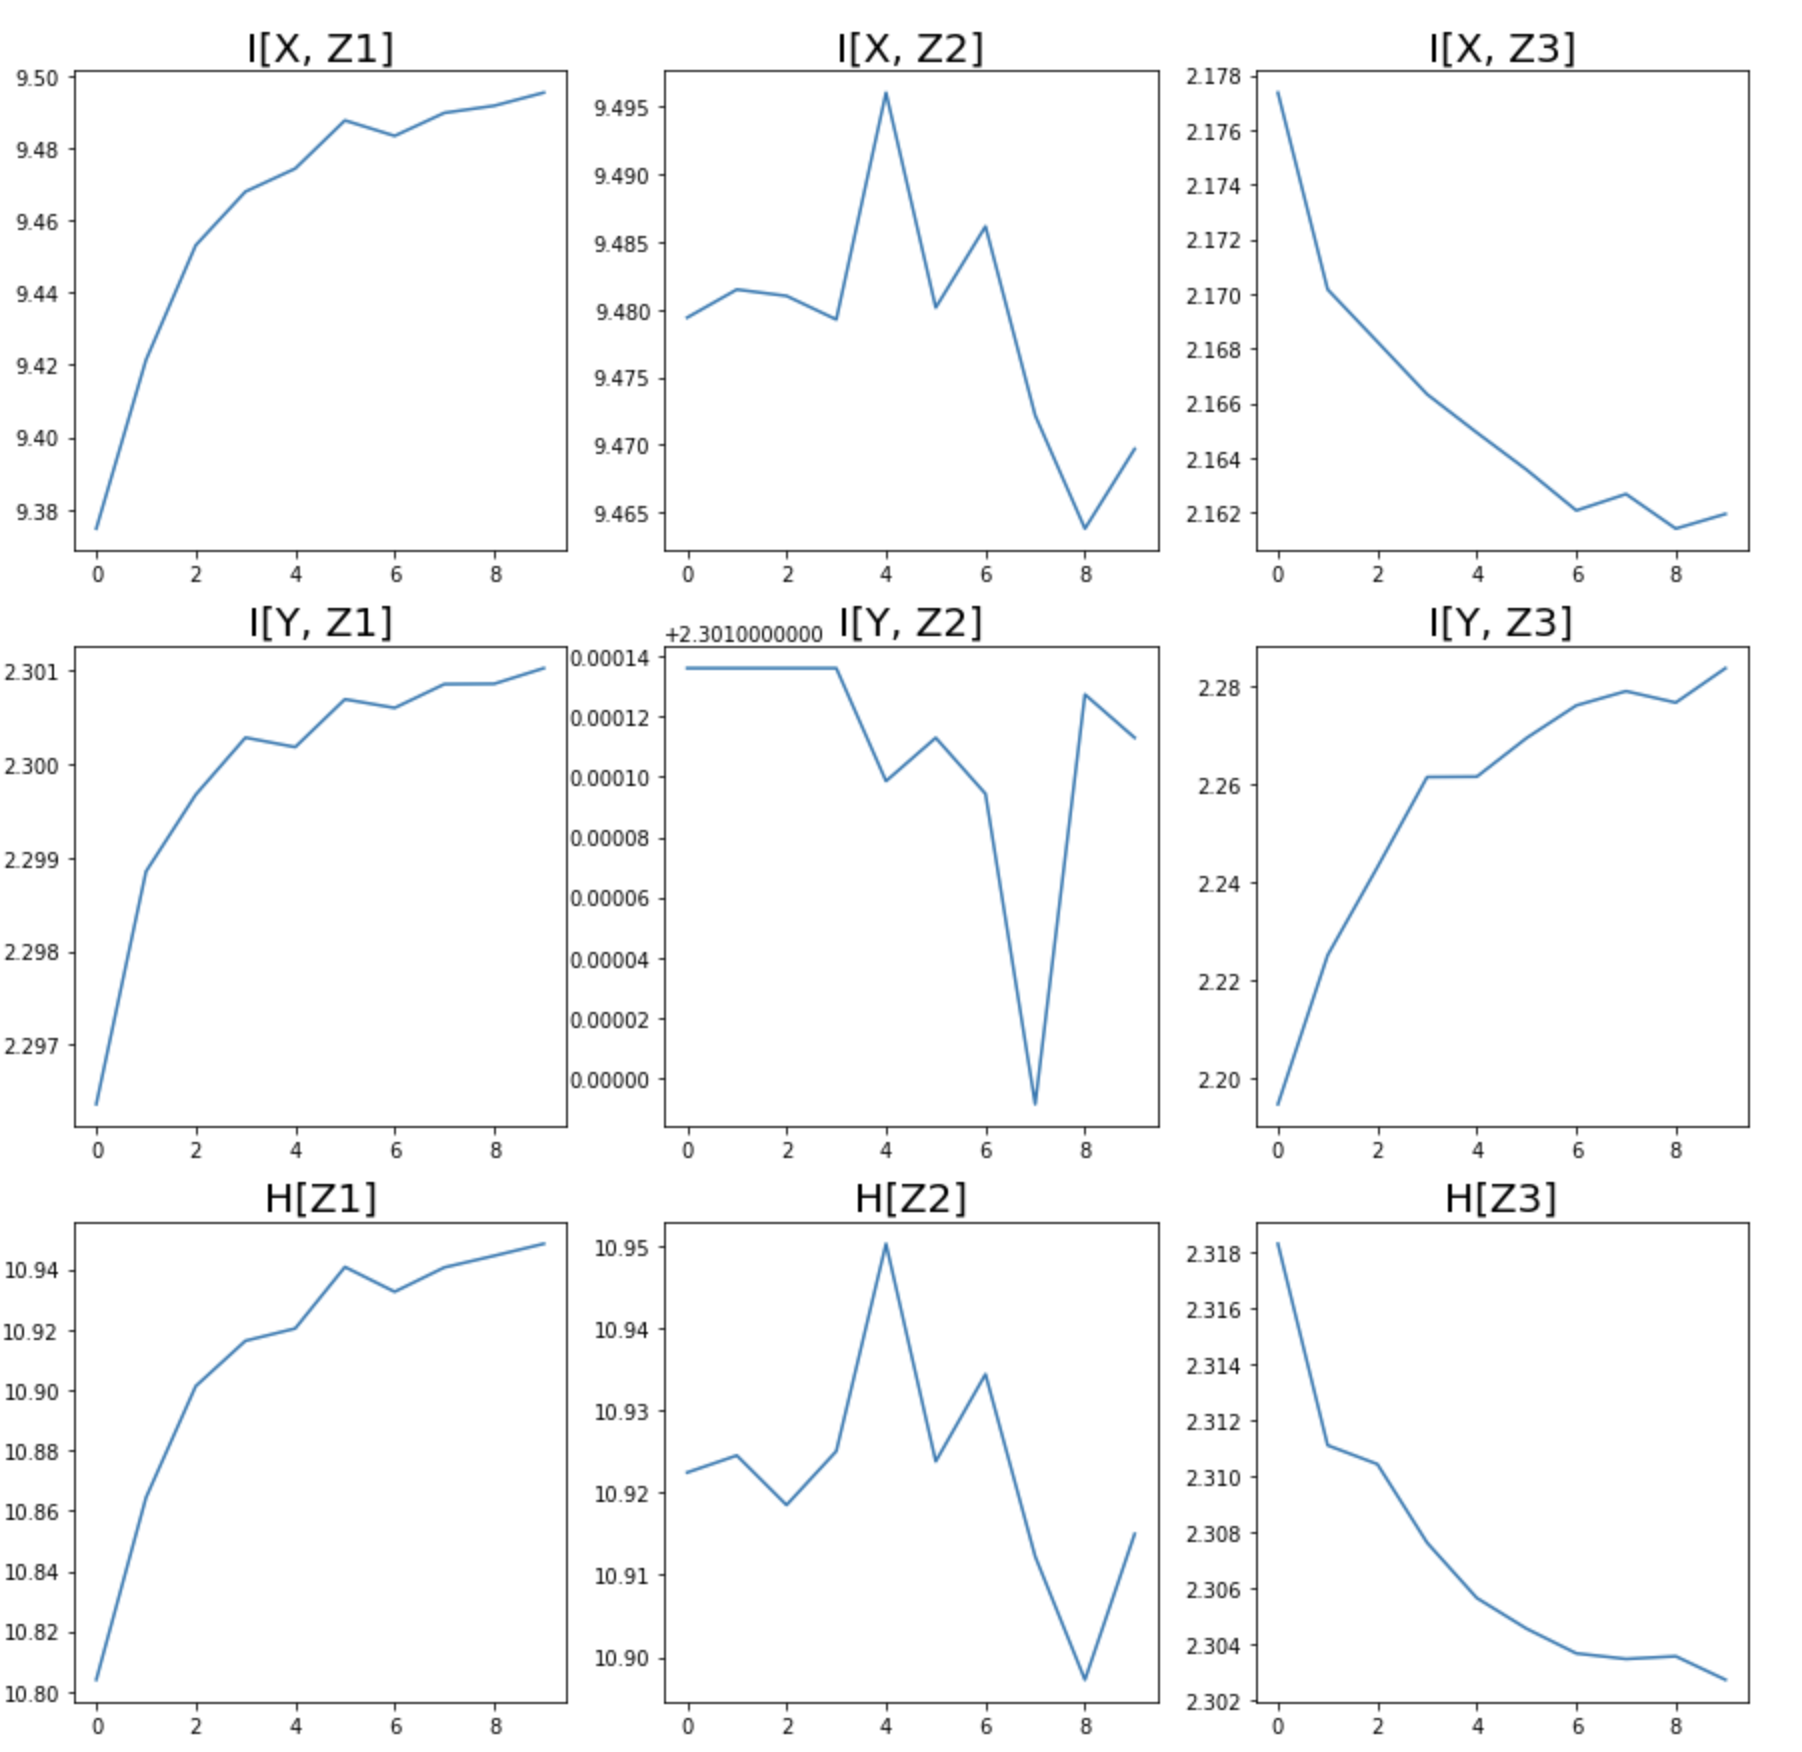
\includegraphics[width=\linewidth]{images/v2.png}
  
\endminipage\hfill
\minipage{0.33\textwidth}
  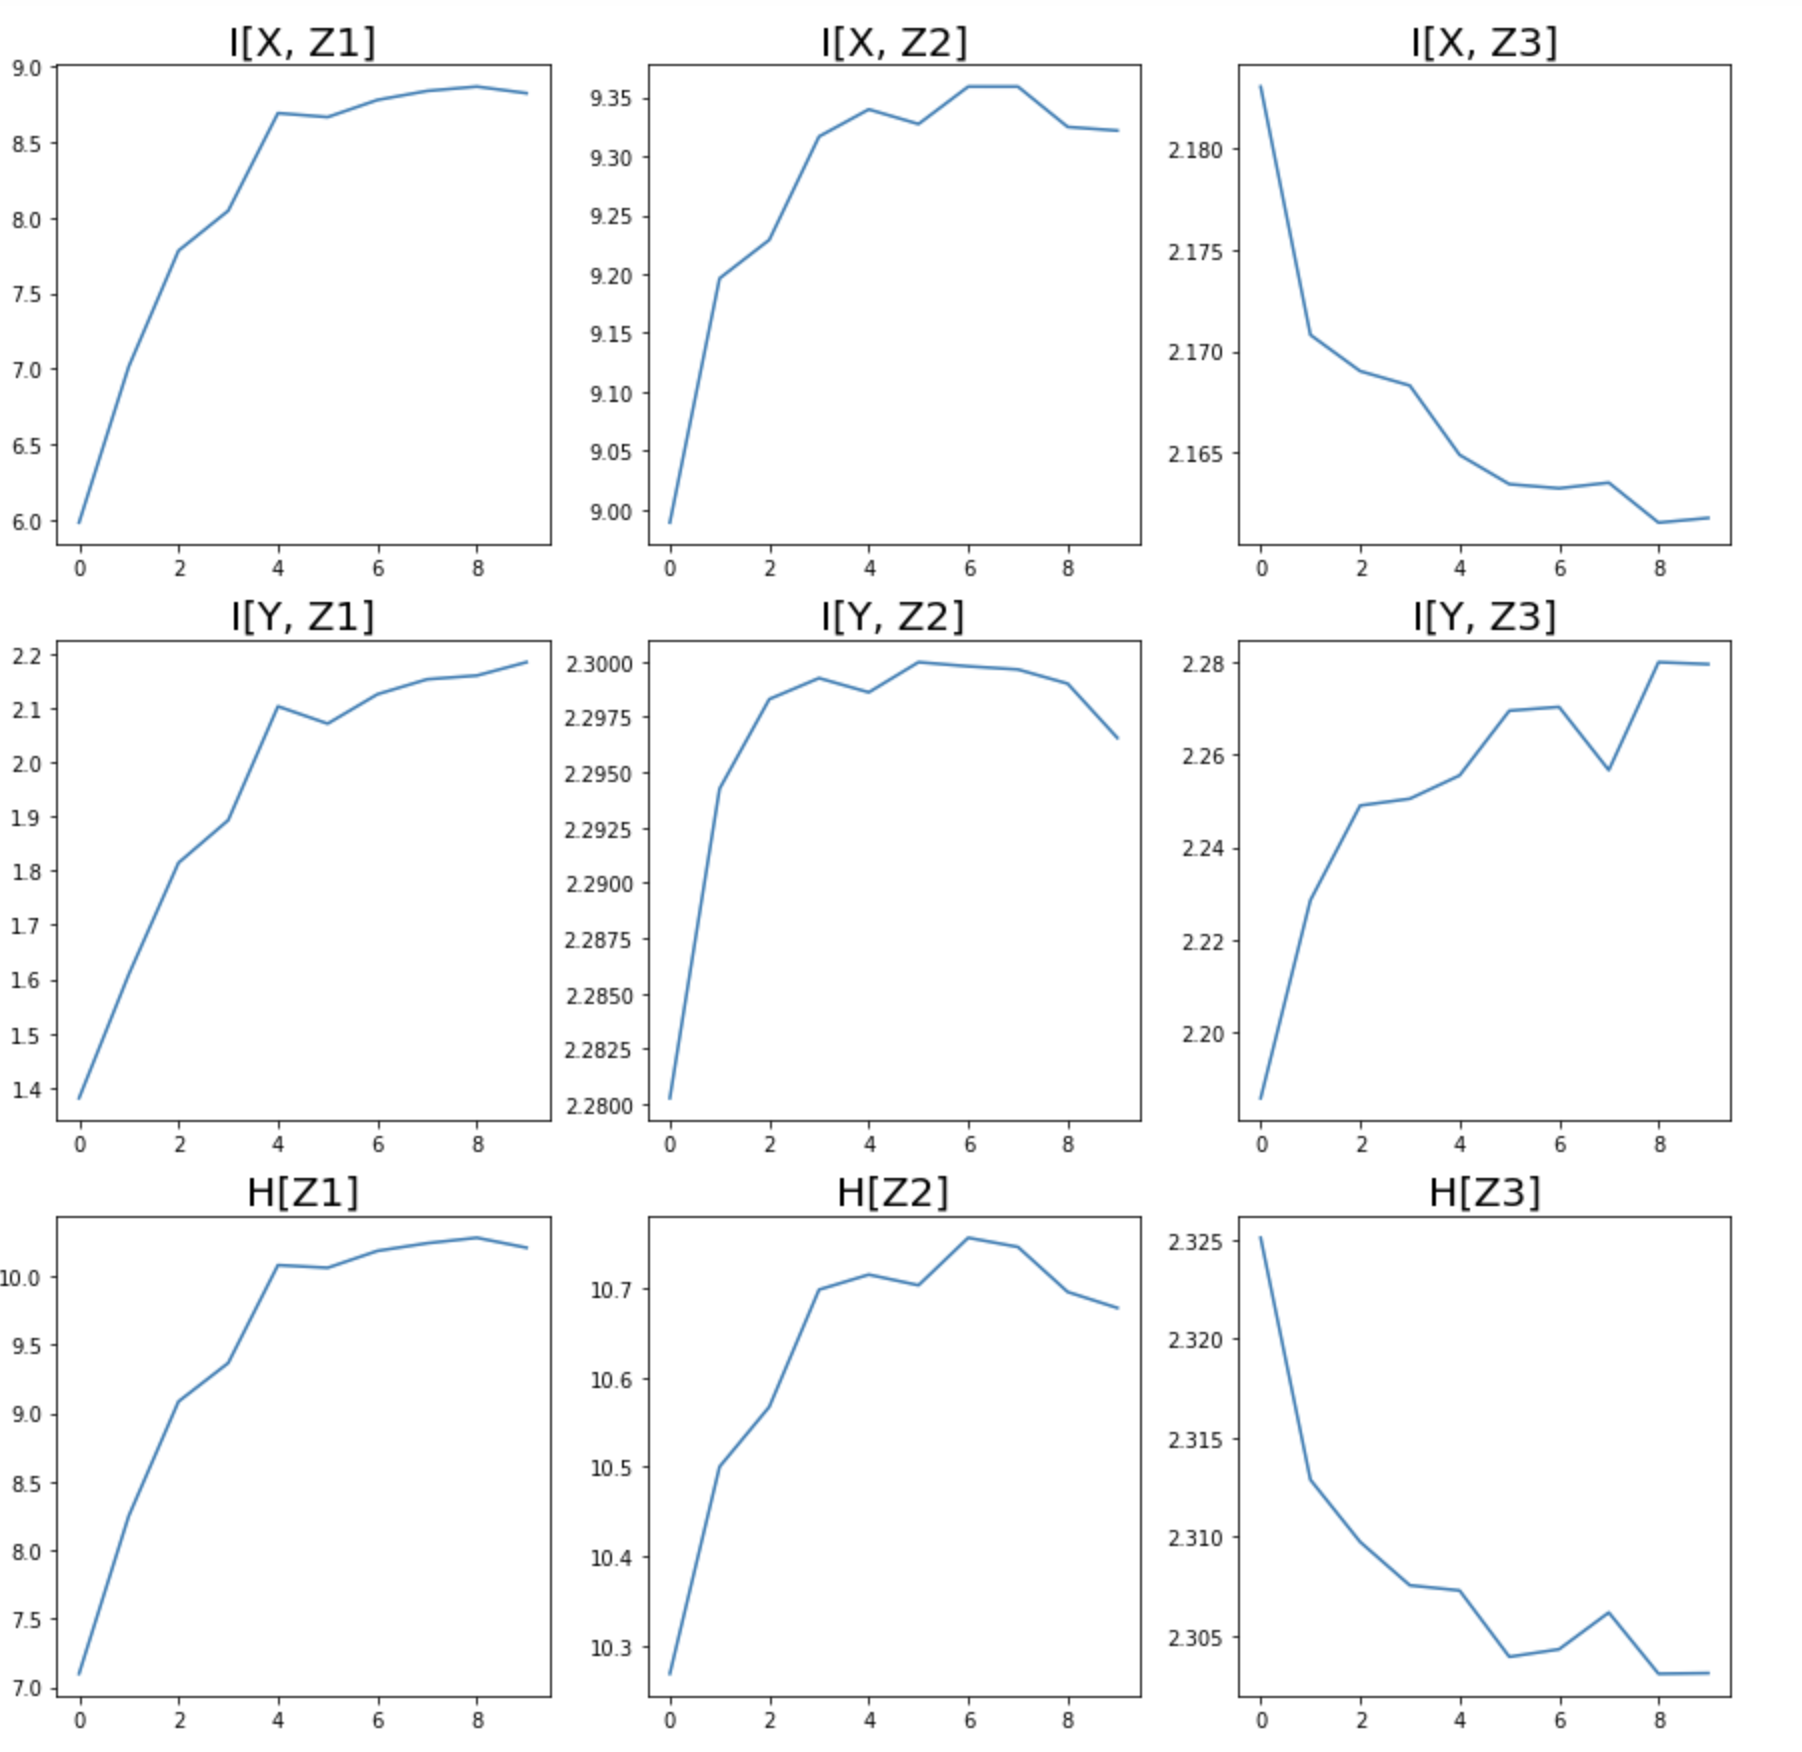
\includegraphics[width=\linewidth]{images/v3.png}
  
\endminipage\hfill
\minipage{0.33\textwidth}
  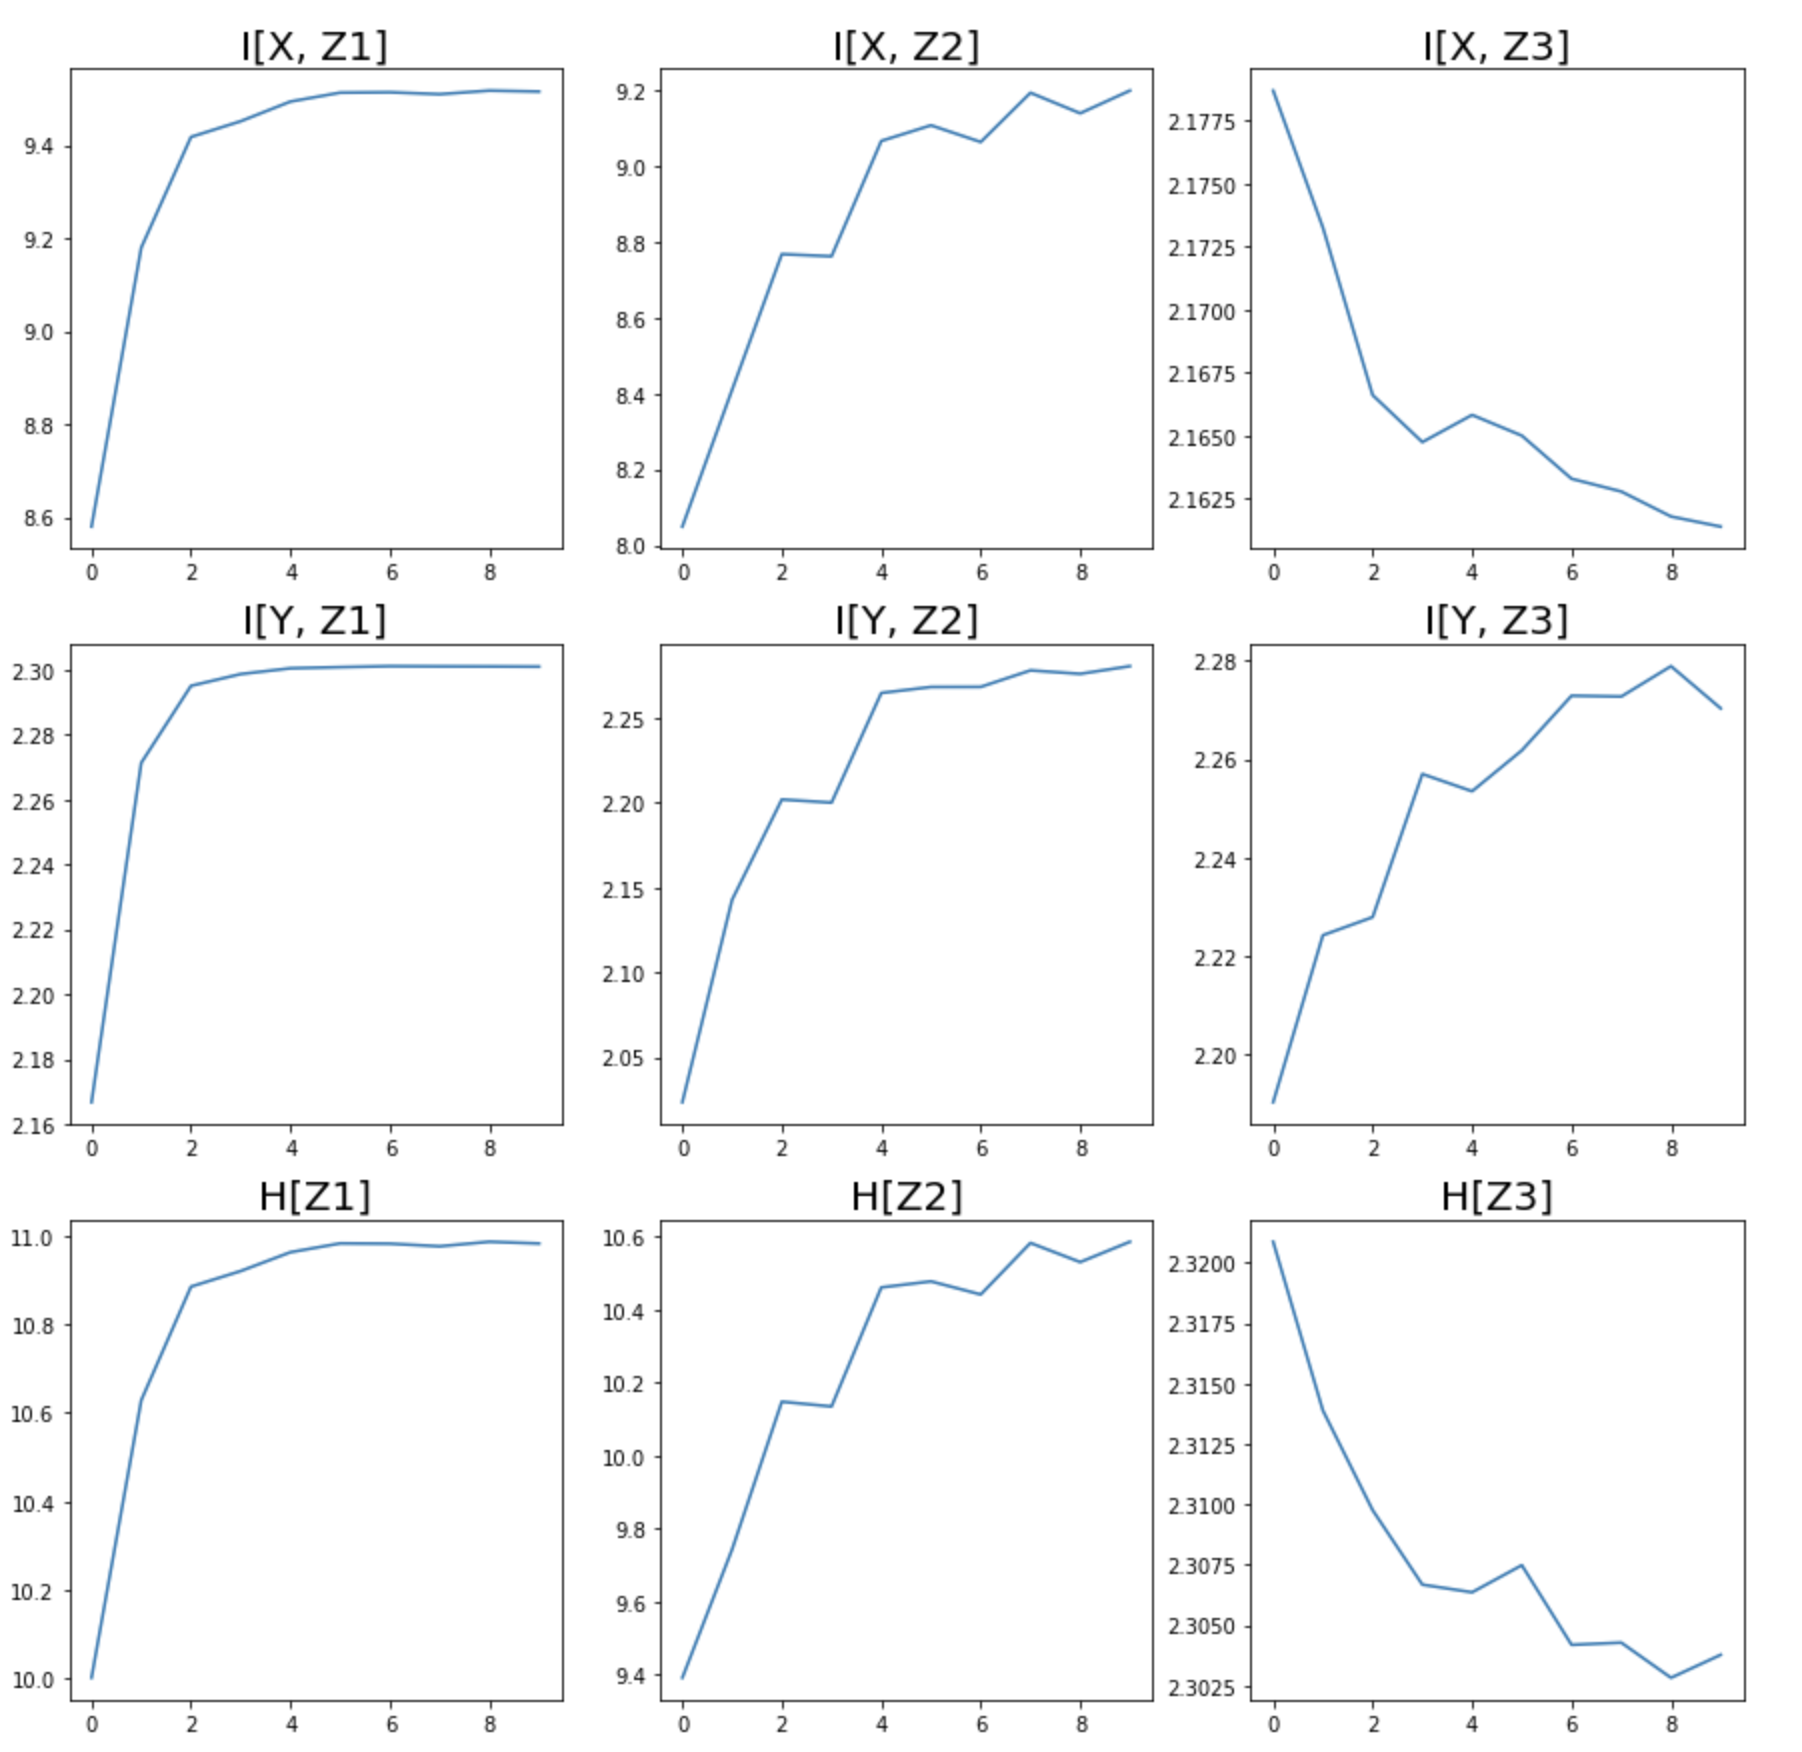
\includegraphics[width=\linewidth]{images/v4.png}
  
\endminipage
\end{figure}
Первое на что стоит обратить внивание - это возрастание метрики $I[X, Z]$ для всех примеров. Аналогично возрастает $I[Z]$. Это происходит по той причине, что значения на латентных слоях в обученных сетках распределены более равномерно. Это происходит по причине, что в необученной сети значения с большим значениями имеют большую вероятность в отличие от значений с маленькими значениями. Это происходит потому что беря максимум по окну с равномерно распределенными значениями максимум будет с большей вероятностью иметь большие значения
\begin{gather}
\begin{aligned}
X_{max} = max(X_1, X_2, ... X_n)
\end{aligned}
\end{gather}
где $X_i$ независимо одинаково распределеные случайные велечины. $X_i \in Uniform(0, 1)$, тогда 
\begin{gather}
\begin{aligned}
p(X_{max} < \alpha) = p(X_1 < \alpha) * ... * p(X_n < \alpha) = \alpha^{n} \rightarrow 0
\end{aligned}
\end{gather}
Соответветственно брав максимум по большому окну со смешанными каналами на плохо обученной сети расределение будет неравномерным. При обучении сети исходные латентные пространства имеют более выраженные предсавления: разрешенная матрица, где ненулевые значения обозначают реакцию на конкретные свертки - соответственно брав максимум по большому окну между несколькими каналами на выходе получится наибольшая реакция на свертку, что имеет равномерное распределение, поэтому с увеличением эпохи энтропия увеличивается и как следствие $H[Z]$ и $I[X, Z]$. Соответственно для данных гиперпараметров метика IB не будет уменьшаться с увеличением эпохи. \\
Для разрешение проблемы неравномерного распределения воспользуемся не maxpooling а avgpooling, то есть будем усреднять а не максимизировать значения в окне. При усреднении неравенство (26) уже не будет действовать, более того среднее у размеренной матрицы стремится к 0, соответственно ситуация с энтропией должны быть симетрична как в прошлом случае. Построим новый пример с нарда новыми гиперпараметрами. \\
4 пример:
\begin{enumerate}
\item $waist\_input = MaxPool2d((4, 4))(input)$
\item $waist\_z1 = ArgPool3d((1, 7, 7))(z1)$
\item $waist\_z2 = ArgPool3d((1, 7, 7))(z2)$
\item $waist\_z3 = Softmax(z3)$
\end{enumerate}
Расмтрим для данного эксперимента полученную информационную маску
\begin{center}
    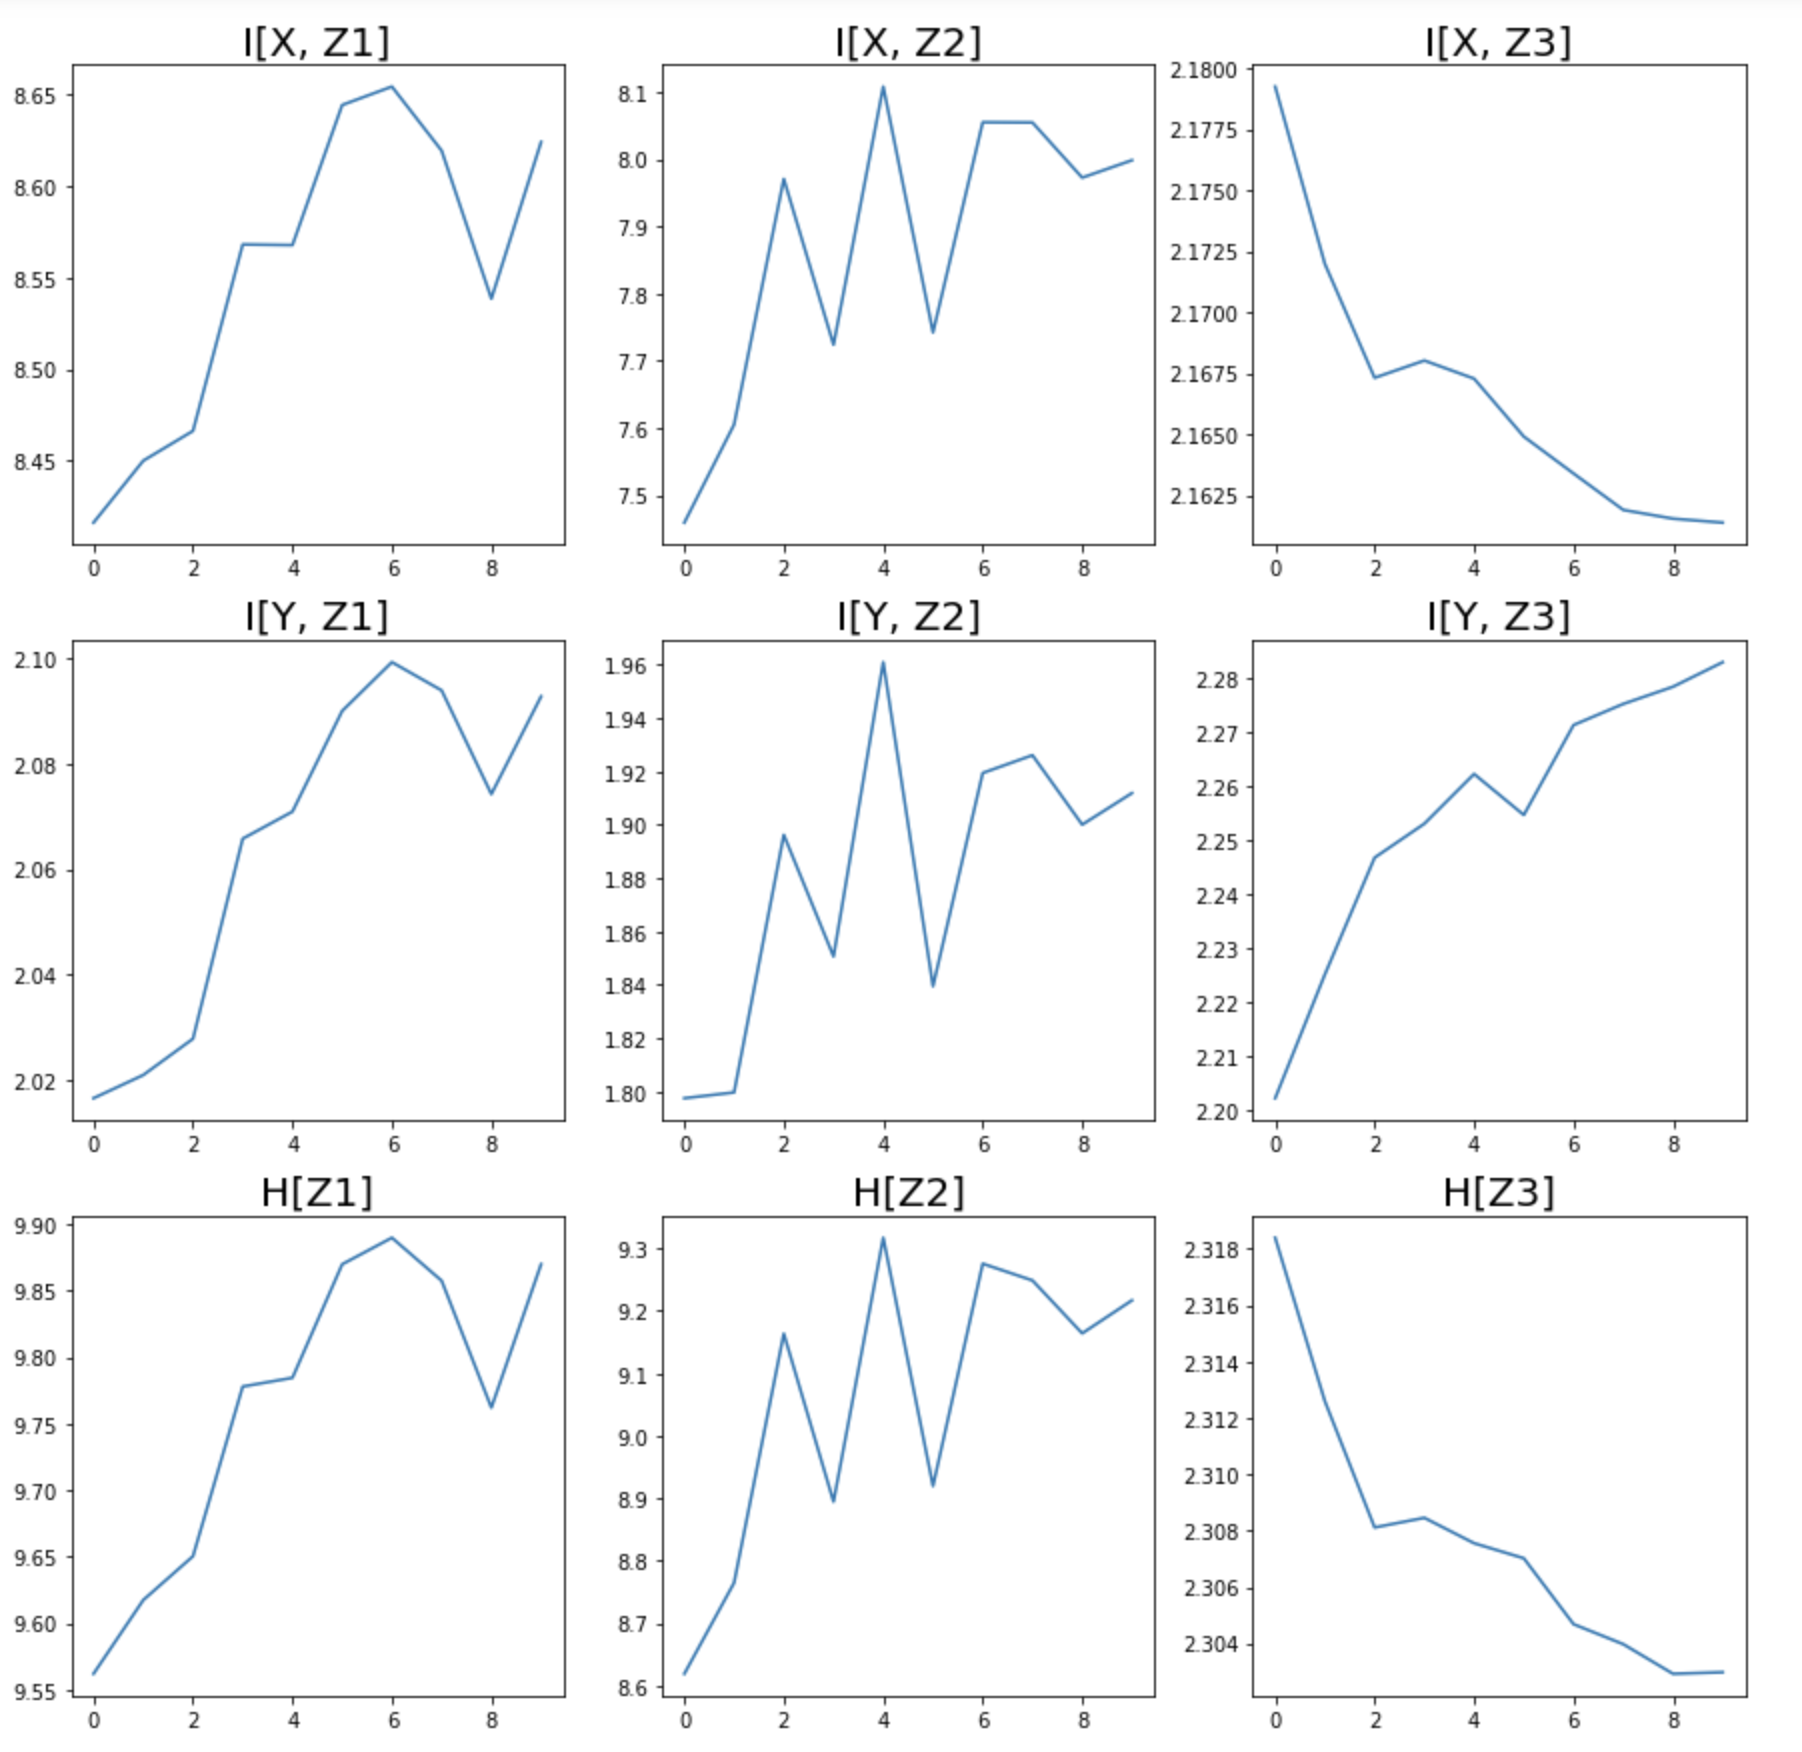
\includegraphics[scale=0.45]{images/v5.png}
\end{center}
Заметим, что возрастание функций $I[X, Z]$ и $I[Z]$ стало менее мнотонно, но при этом общий характер возрастания при увеличении эпохи остался, что требует большего изучения.

\newpage
\section{Заключение}
Сделаем выводы о проведенных экспериментах. Изначально мы пришли к выводу что задача обучения нейронной сети это решение оптимизационной задачи
\begin{gather}
\begin{aligned}
min_{Z} I[X, Z] - \beta * I[Z, Y]
\end{aligned}
\end{gather}
То есть мы хотим минимизировать взаимную информацию между входным  пространством и латентным, при этом максимизовать общую информацию между выходом и латентым пространством. Изначально мы хотели проверить насколько эта гипотеза верна на практике. \\
Тезисно приведем выводы которые были сделаны на протяжение работы:
\begin{enumerate}
\item Рассмотрев слои, был сделан вывод, что значения по отдельным признакам зависят друг от друга, также значения по каждому признаку распредедены нестандартно, поэтому сузим пространства до дискретных и вероятностнь будем оценивать количественно.
\item Сужение должно быть оптимальным, а именно быть не инъективнм, чтобы не быть равномернораспределеным и изменятся от эпохи к эпохе, при этом сохранять информацию о изначальном пространстве.
\item Для сужений принято решение использовать конкатенацию пуллингов и дискретизацию, при этом на выходном слое использовать softmax.
\item Доказано что при сужении не достаточно использовать только дискретизацию, так как размерность полученных пространств слишком большая из-за чего отображение получается инъективно и операция построения вероятностоного пространства слишком долгая.
\item В качестве операции понижения размерности пуллинги сохраняют информацию, так как операция пуллинг часто используется как слои в нейронных сетях для понижения размерности, соответственно через них проходит нужжная информация.
\item Всего в сети 3 латентных пространства, которые последовательно упрощаются, чем сложнее пространство тем более непредстказуемо ведут себя информационные метрики на них.
\item Финальное латентное пространство подтверждает выдвинутую в начале гипотезу и для этого пространства метрика $I[X, Z]$ уменьшается, а $I[Y, Z]$ увеличивается с эпохой обучения, а значит общая метрика (27) (Information Bottleneck) также будет уменьшаться с эпохой.
\item При этом информационнык метрики на первых латентных пространствах ведут себя непредсказуемо. Если уменьшать пространство немного, то метрики либо меняются очень слабо либо хаотично, что говорит о инъективности сужения. При этом сжав слишком сильно пространство все информационные метрики: $I[X, Z]$, $I[Y, Z]$, $H[Z]$ увеличиваются с эпохой обучения.
\item Одна из причин поведения в предъиущем пункте - несохранения распределения значений при пуллинге, то есть при обучении латентное пространство становится более равномерно распределенным, отчешл все метрики возрастают, данная проблема требует дополнительного исследования.
\end{enumerate}

В данной работе были подробно рассмотрены поведения информационных метрик в динамике обучения модели, в частности была подробна рассмотрена небольшая свертночная нейронная сеть, подробно рассмотрено поведение различных слоев данной сети и статистически оценено с вероятностной точки зрения. Также в данной работе построен универсальный способ подсчета информации отдельных слоев так и совместной информации для любого состояния любой нейронной сети. Была четко поставлена гипотеза, построенная на теоретических знаниях из релевантной литературы и проверена в действии на практике.


\newpage
\section{Заключение}
Сделаем выводы о проведенных экспериментах. Изначально мы пришли к выводу что задача обучения нейронной сети это решение оптимизационной задачи
\begin{gather}
\begin{aligned}
min_{Z} I[X, Z] - \beta * I[Z, Y]
\end{aligned}
\end{gather}
То есть мы хотим минимизировать взаимную информацию между входным  пространством и латентным, при этом максимизовать общую информацию между выходом и латентым пространством. Изначально мы хотели проверить насколько эта гипотеза верна на практике. \\
Тезисно приведем выводы которые были сделаны на протяжение работы:
\begin{enumerate}
\item Рассмотрев слои, был сделан вывод, что значения по отдельным признакам зависят друг от друга, также значения по каждому признаку распредедены нестандартно, поэтому сузим пространства до дискретных и вероятностнь будем оценивать количественно.
\item Сужение должно быть оптимальным, а именно быть не инъективнм, чтобы не быть равномернораспределеным и изменятся от эпохи к эпохе, при этом сохранять информацию о изначальном пространстве.
\item Для сужений принято решение использовать конкатенацию пуллингов и дискретизацию, при этом на выходном слое использовать softmax.
\item Доказано что при сужении не достаточно использовать только дискретизацию, так как размерность полученных пространств слишком большая из-за чего отображение получается инъективно и операция построения вероятностоного пространства слишком долгая.
\item В качестве операции понижения размерности пуллинги сохраняют информацию, так как операция пуллинг часто используется как слои в нейронных сетях для понижения размерности, соответственно через них проходит нужжная информация.
\item Всего в сети 3 латентных пространства, которые последовательно упрощаются, чем сложнее пространство тем более непредстказуемо ведут себя информационные метрики на них.
\item Финальное латентное пространство подтверждает выдвинутую в начале гипотезу и для этого пространства метрика $I[X, Z]$ уменьшается, а $I[Y, Z]$ увеличивается с эпохой обучения, а значит общая метрика (27) (Information Bottleneck) также будет уменьшаться с эпохой.
\item При этом информационнык метрики на первых латентных пространствах ведут себя непредсказуемо. Если уменьшать пространство немного, то метрики либо меняются очень слабо либо хаотично, что говорит о инъективности сужения. При этом сжав слишком сильно пространство все информационные метрики: $I[X, Z]$, $I[Y, Z]$, $H[Z]$ увеличиваются с эпохой обучения.
\item Одна из причин поведения в предъиущем пункте - несохранения распределения значений при пуллинге, то есть при обучении латентное пространство становится более равномерно распределенным, отчешл все метрики возрастают, данная проблема требует дополнительного исследования.
\end{enumerate}

В данной работе были подробно рассмотрены поведения информационных метрик в динамике обучения модели, в частности была подробна рассмотрена небольшая свертночная нейронная сеть, подробно рассмотрено поведение различных слоев данной сети и статистически оценено с вероятностной точки зрения. Также в данной работе построен универсальный способ подсчета информации отдельных слоев так и совместной информации для любого состояния любой нейронной сети. Была четко поставлена гипотеза, построенная на теоретических знаниях из релевантной литературы и проверена в действии на практике.


\begin{thebibliography}{9}
\bibitem{texbook}
Andreas Kirsch, Clare Lyle, Yarin Gal (2021) \emph{Unpacking Information Bottlenecks: Surrogate Objectives for Deep Learning}, Department of Computer Science University of Oxford

\bibitem{texbook}
Naftali Tishby, Noga Zaslavsky (2015) \emph{Deep Learning and the Information Bottleneck Principle}
\end{thebibliography}
\end{document}
